\documentclass{beamer}
%\documentclass[aspectratio=169]{beamer}

\usetheme{metropolis}
\usepackage{xcolor}
%\usepackage[sfdefault,light]{FiraSans}
%\usepackage[sfdefault]{FiraSans}

\usepackage{comfortaa}
\usepackage{roboto}
\usepackage[T1]{fontenc}

\usepackage{braket}
\usepackage{qrcode}
\usepackage{tabularx}
\usepackage{siunitx}


% adjust fonts and colors

\setbeamerfont{title}{family=\comfortaa\scshape}
\setbeamerfont{section title}{family=\comfortaa\scshape}
\setbeamerfont{frametitle}{family=\comfortaa\scshape}
\setbeamerfont{titlelike}{family=\comfortaa\scshape}
\setbeamerfont{block title}{family=\comfortaa\scshape}
\setbeamerfont{block title example}{family=\comfortaa\scshape}
\setbeamerfont{block title alerted}{family=\comfortaa\scshape}
\setbeamerfont{caption name}{family=\comfortaa\scshape}
\setbeamerfont{normal text}{family=\roboto\scshape}

\definecolor{wuespacepurple}{rgb}{0.2705,0.1569,0.59215}

\setbeamercolor{frametitle}{fg=wuespacepurple}
\setbeamercolor{section title}{fg=white}
\setbeamercolor{titlelike}{fg=wuespacepurple}
\setbeamercolor{background canvas}{bg=white}

% links without color
\hypersetup{colorlinks=false}

% change style of blocks
\metroset{block=fill}
\setbeamercolor{block title}{fg=wuespacepurple}
\setbeamercolor{block title alerted}{fg=myred}
\setbeamercolor{block title example}{fg=mygreen}

\setbeamercolor{progress bar}{fg=orange,bg=lightgray}

% blue background in section slides
\AtBeginSection{
    {
    \setbeamercolor{background canvas}{bg=wuespacepurple}
    \frame[plain,c,noframenumbering]{
      \sectionpage
%      \tableofcontents[hideothersubsections,sectionstyle=hide,subsectionstyle=shaded/shaded/hide]
    }
  }
}

\makeatletter
\setlength{\metropolis@titleseparator@linewidth}{2pt}
\setlength{\metropolis@progressonsectionpage@linewidth}{2pt}
\setlength{\metropolis@progressinheadfoot@linewidth}{2pt}
\makeatother


% itemize symbols
\setbeamertemplate{itemize subitem}{-}
\setbeamertemplate{itemize subsubitem}{$\cdot$}

% numbered sections in table of contents
\setbeamertemplate{section in toc}[sections numbered]
%\setbeamertemplate{subsection in toc}[subsections numbered]
\setbeamertemplate{subsection in toc}{\hspace{1.2em}-~\inserttocsubsection\par}

% adjust frame title (with page numbers and a smaller spacing to the following content)
\defbeamertemplate*{frametitle}{wuespaceframetitle}{%
	% Is there a more elegenat way of putting the logo at the right place, e.g., remove borders?
	\vspace{-0.039cm}
  \ifratio{169}{
    \hspace{-1.112cm}
    \parbox{1.24cm}{
      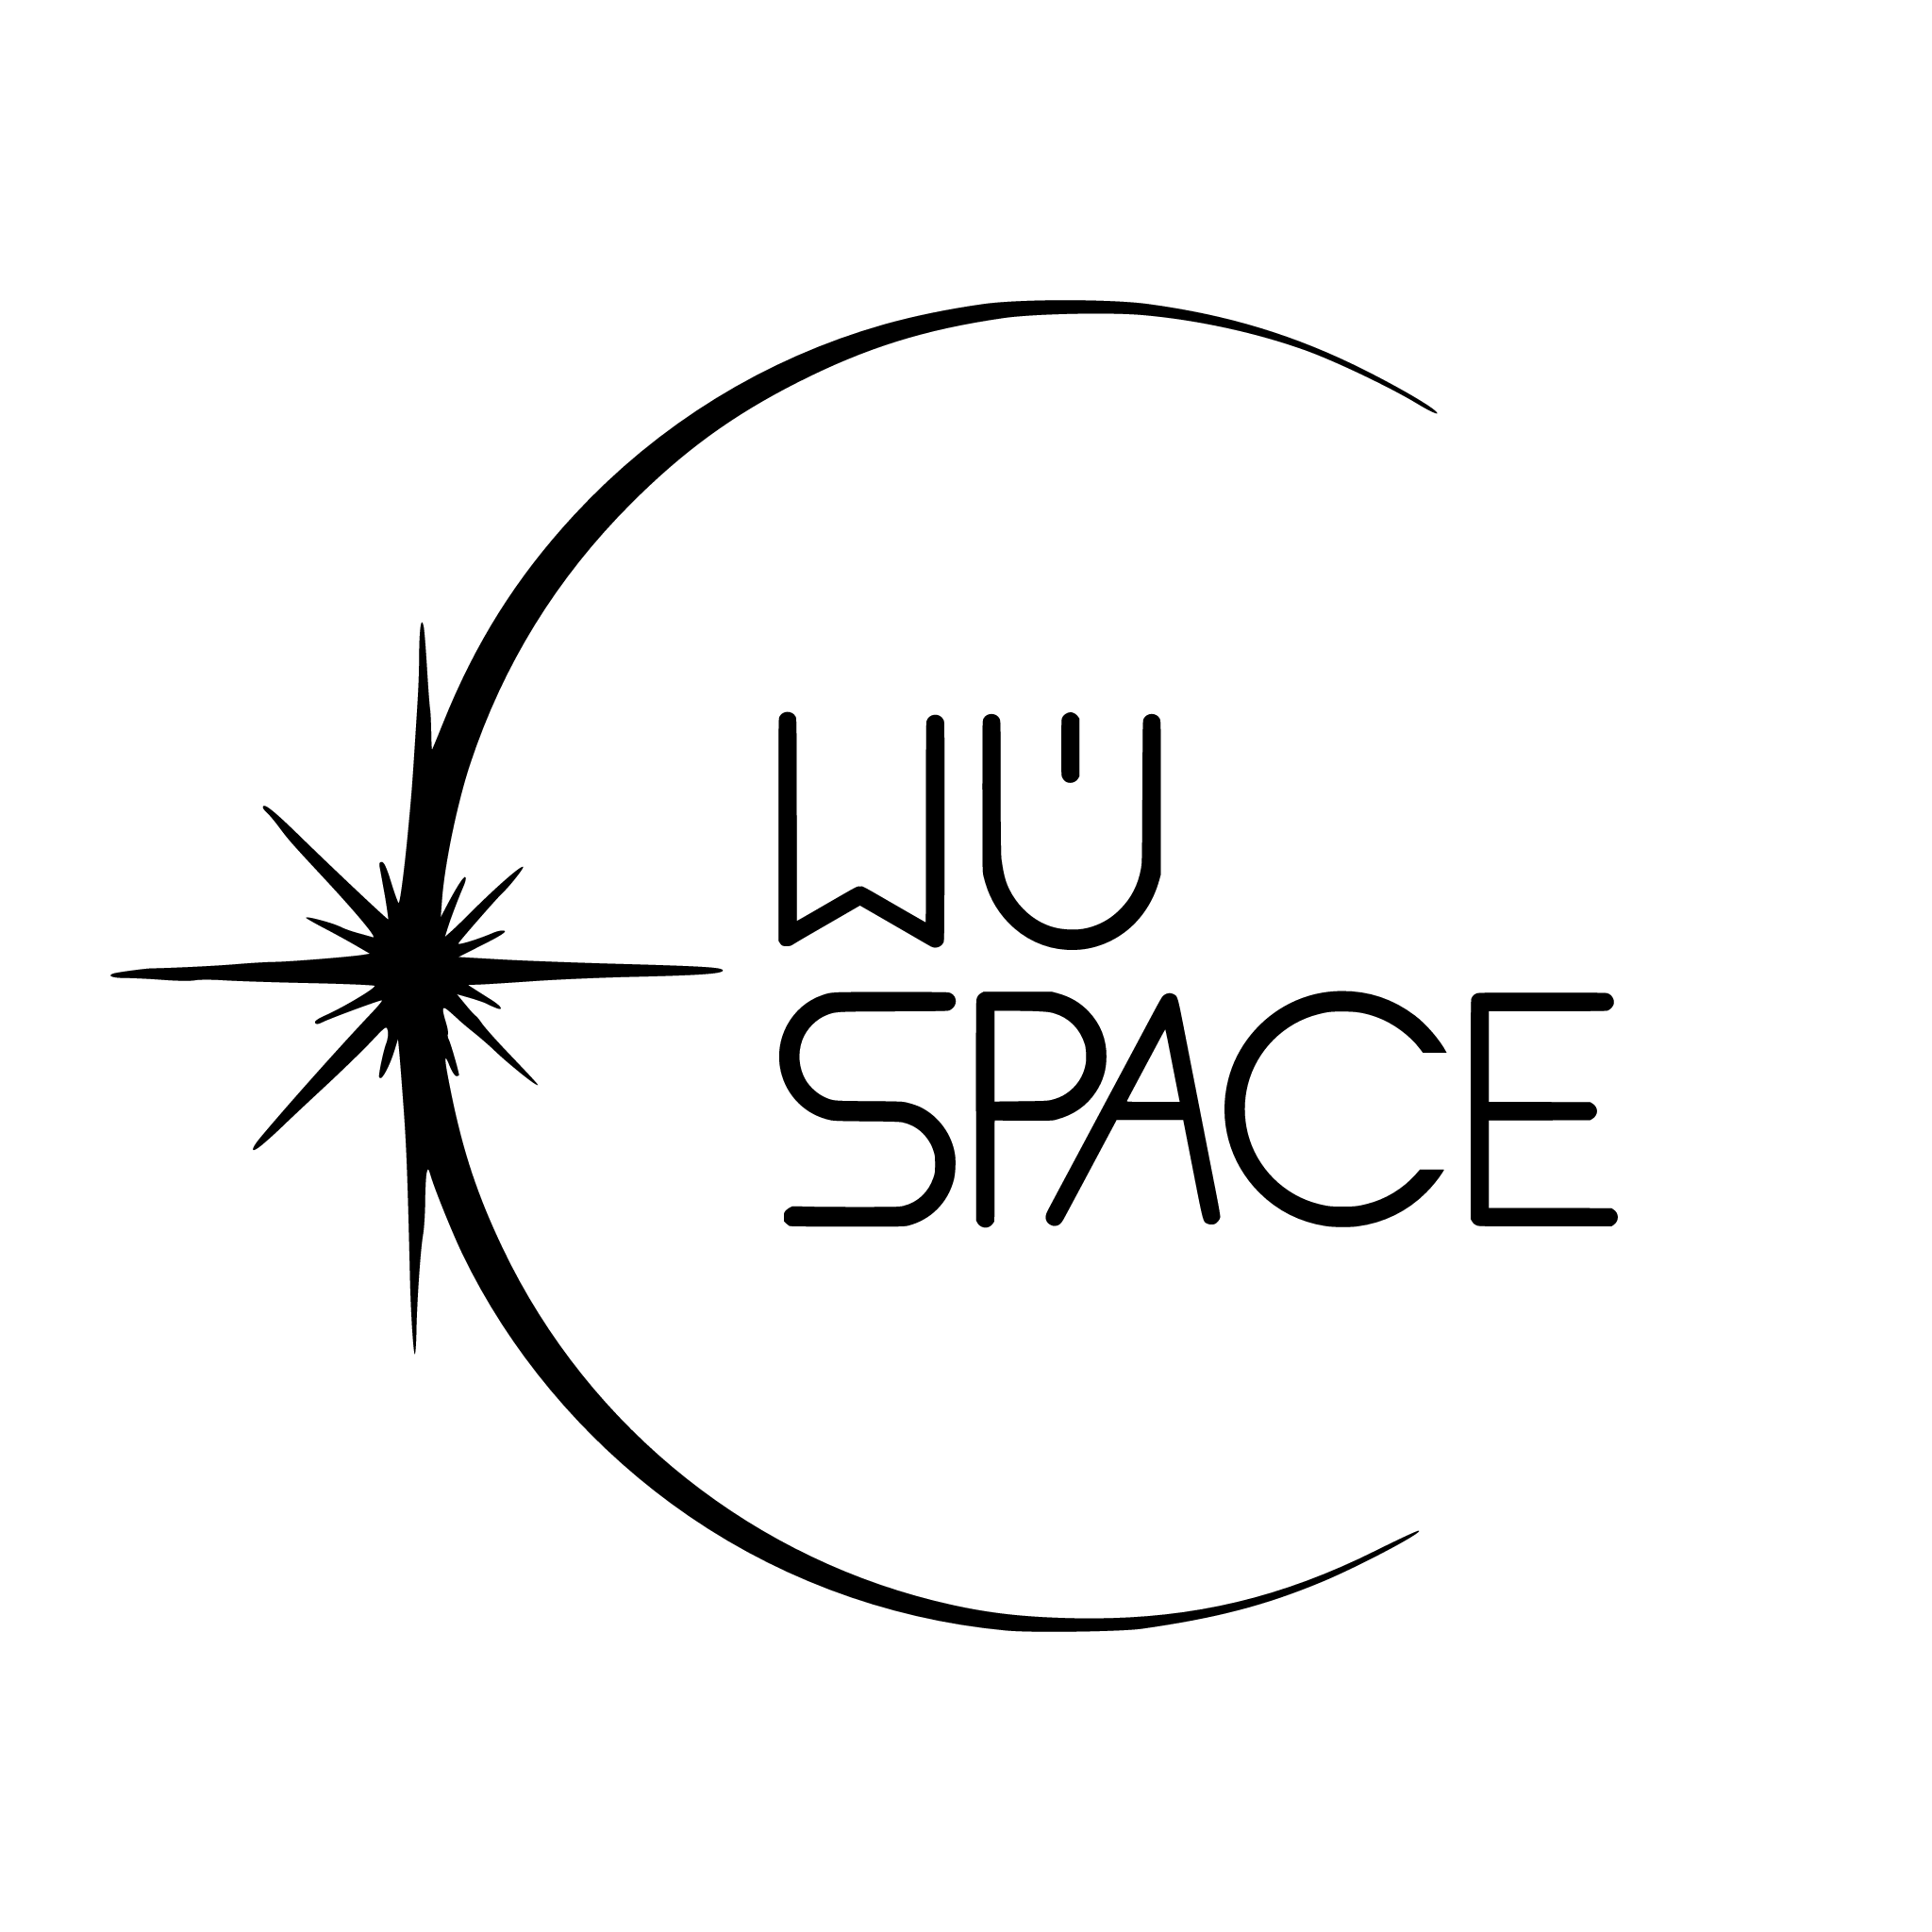
\includegraphics[width=1.24cm,keepaspectratio]{wuespace-small.png}
    }
  }{
    \hspace{-1.12cm}
    \parbox{1.3cm}{
      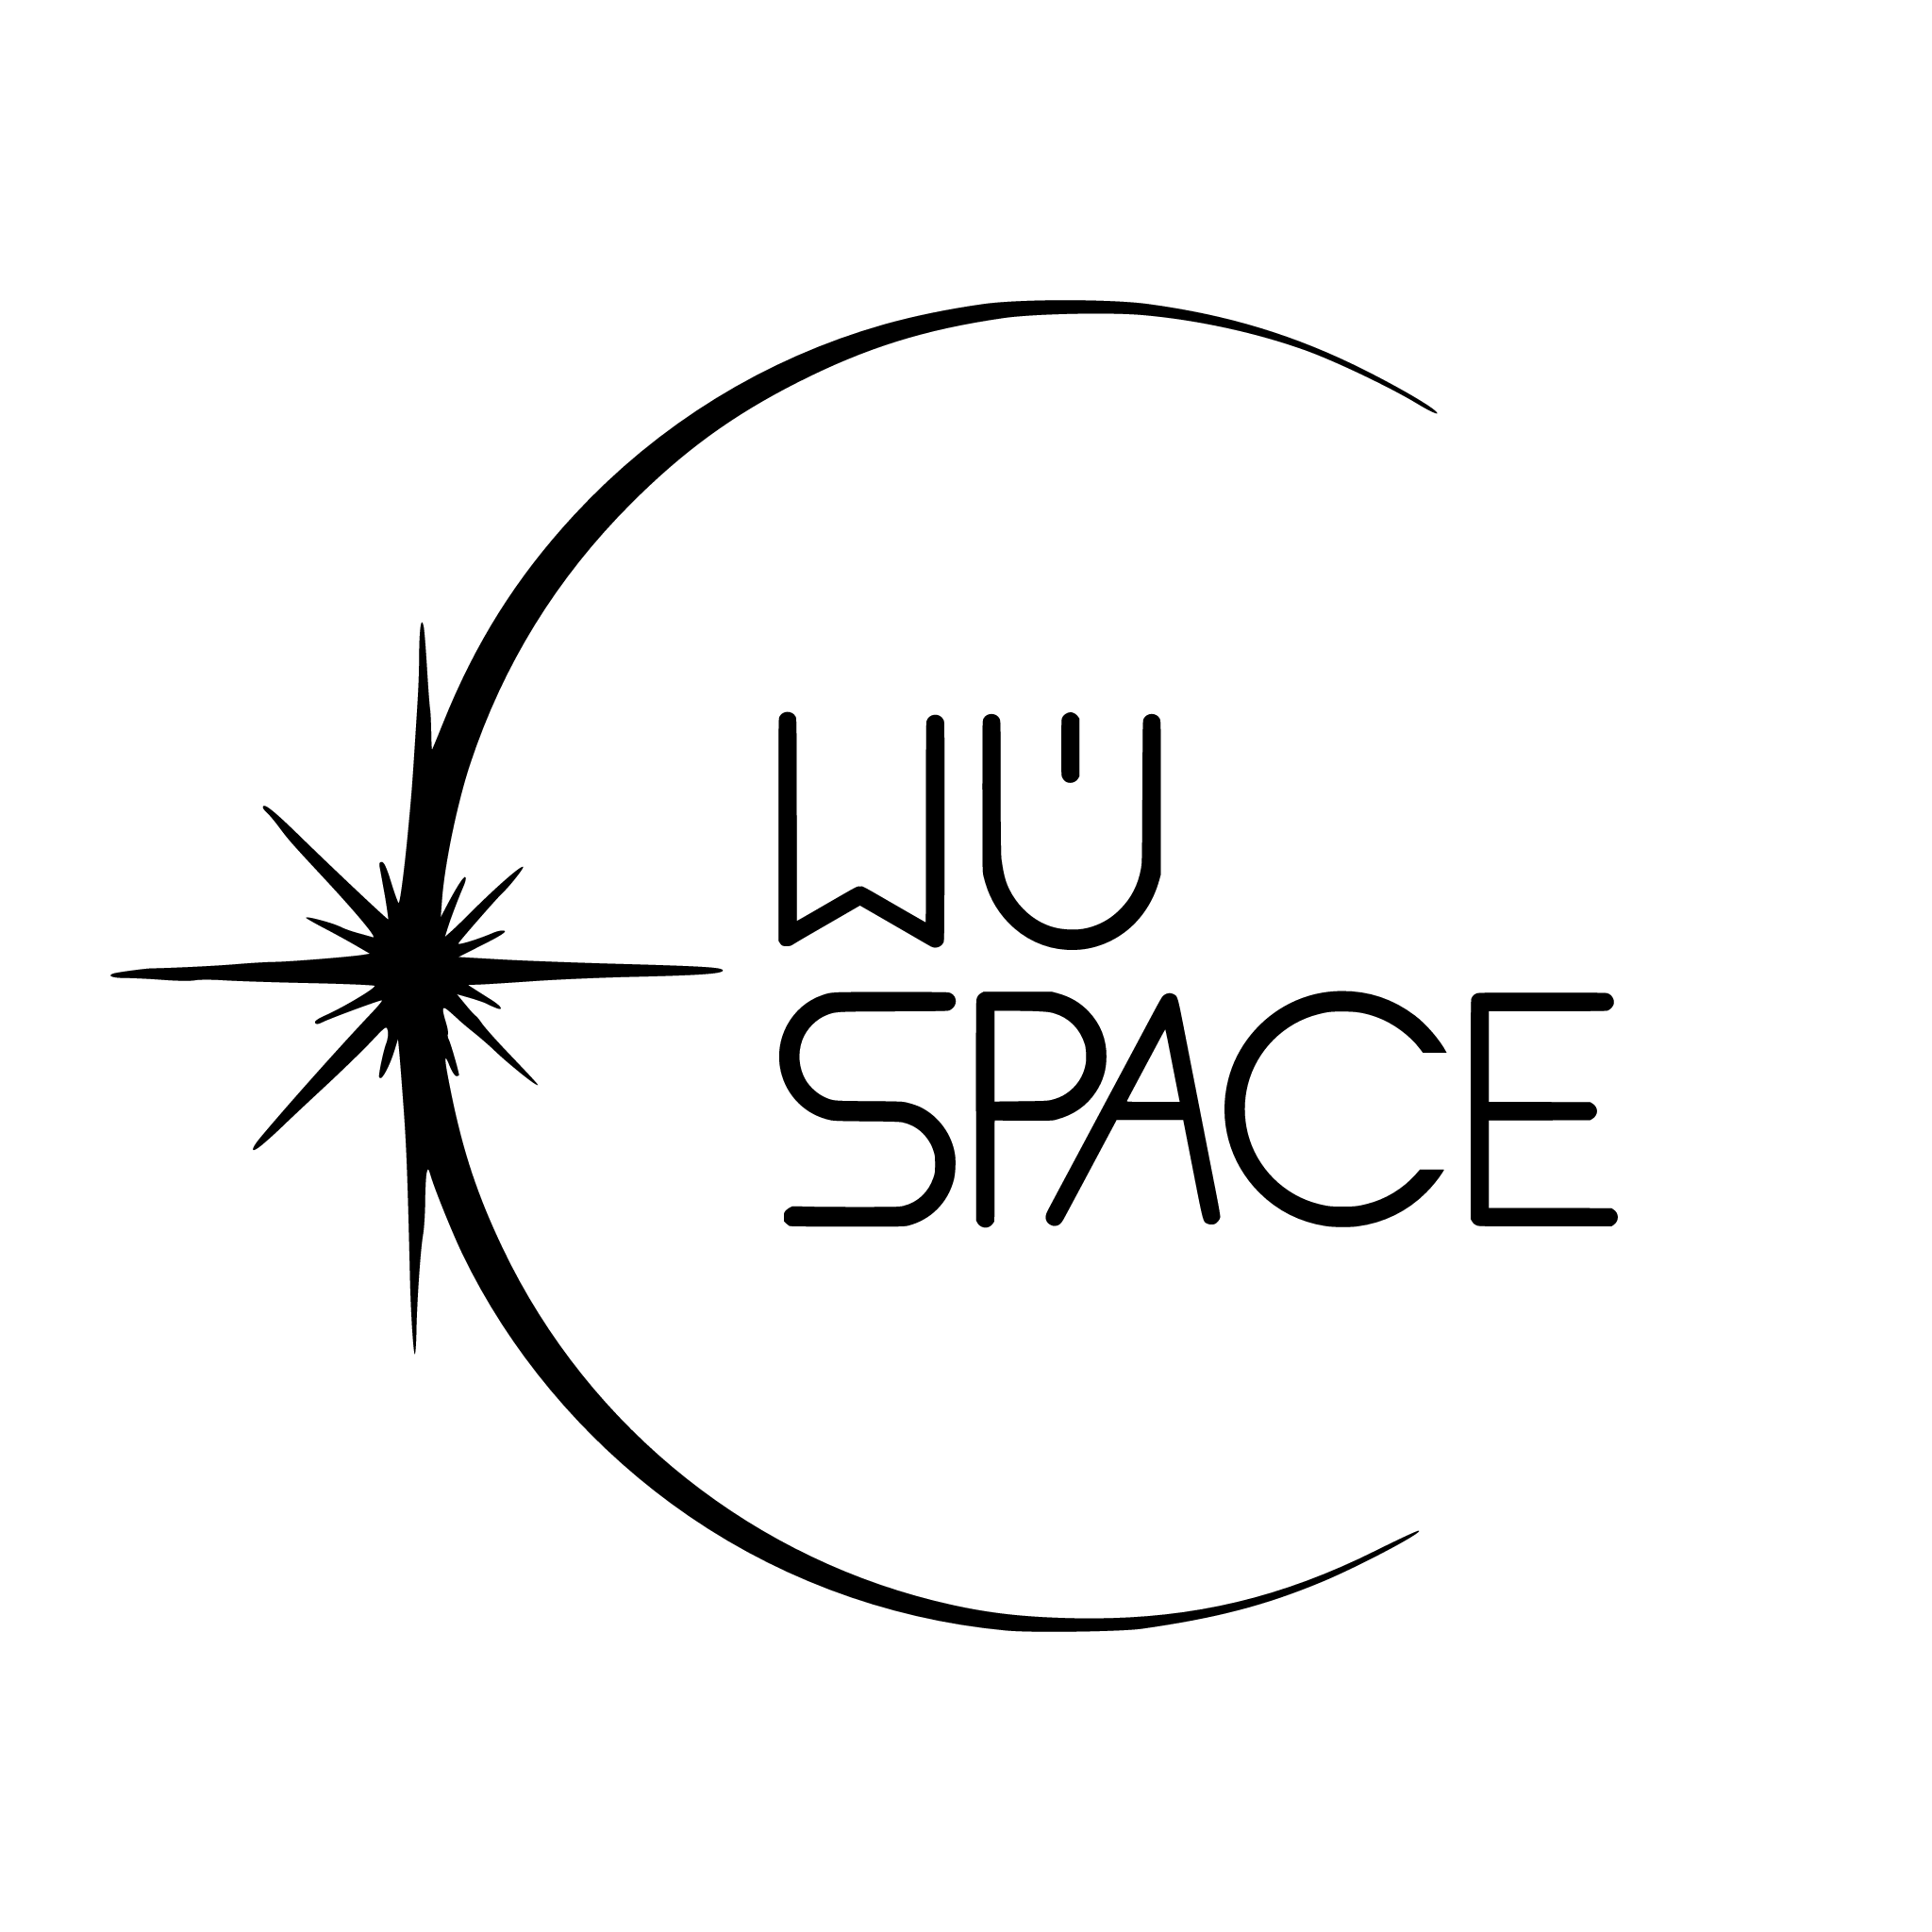
\includegraphics[width=1.2cm,keepaspectratio]{wuespace-small.png}
    }
  }
  \hspace{.1cm}
  \parbox{9.9cm}{\insertframetitle}%
}

\setbeamertemplate{frametitle}[wuespaceframetitle]

\defbeamertemplate*{footline}{wuespacefootline}{
  \ifnum \theframenumber=1
  \else
    \centering
    \parbox{.97\paperwidth}{
      \mbox{\insertshortauthor: \insertshorttitle}, \insertshortinstitute, \insertshortdate \hfill \insertframenumber}
    \vskip.8em
  \fi
}

\setbeamertemplate{footline}[wuespacefootline]

\makeatletter
\newcommand\ifratio[3]{%
\ifnum#1=169%
    \ifdim\beamer@paperwidth=16.00cm\relax%
        \ifdim\beamer@paperheight=9.00cm\relax%
            #2%
        \else%
            #3%
        \fi%
    \else%
        #3%
    \fi%
\else%
    \ifnum#1=43%
        \ifdim\beamer@paperwidth=12.80cm\relax%
            \ifdim\beamer@paperheight=9.60cm\relax%
                #2%
            \else%
                #3%
            \fi%
        \else%
            #3%
        \fi%
    \fi%
\fi%
}
\makeatother

% define title page
\defbeamertemplate*{background canvas}{titlepage}
{
  \ifratio{169}{
    \hspace*{0.93cm}
  }{
    \hspace*{0.748cm}
  }
  \color{wuespacepurple}\vrule width\paperwidth height\paperheight% added bg color
}

\setbeamertemplate{title page}{
  \hspace*{.9cm}
  \centering
  \begin{minipage}[c][.8\paperheight]{.8\textwidth}
    \ifx\inserttitle\@empty\else\usebeamertemplate*{title}\fi
    \ifx\insertsubtitle\@empty\else\usebeamertemplate*{subtitle}\fi
    \usebeamertemplate*{title separator}
    \ifx\beamer@shortauthor\@empty\else\usebeamertemplate*{author}\fi
    \ifx\insertdate\@empty\else\usebeamertemplate*{date}\fi
    \ifx\insertinstitute\@empty\else\usebeamertemplate*{institute}\fi
  \end{minipage}
}



\newcommand\Wider[2][3em]{%
\makebox[\linewidth][c]{%
  \begin{minipage}{\dimexpr\textwidth+#1\relax}
  \raggedright#2
  \end{minipage}%
  }%
}

\AtBeginSubsection
{
    \begin{frame}   
        \frametitle{Contents}
        \tableofcontents[currentsection,currentsubsection,subsectionstyle=show/shaded/hide]
    \end{frame}
}

\usepackage{amsmath}
\usepackage[normalem]{ulem}
\usepackage{booktabs,array}
\usepackage{animate}

\usepackage[english]{babel}

\usepackage{anyfontsize}
\usepackage{subfig}

\usepackage{multicol}

\usepackage{tikz}
\usetikzlibrary{calc,shadings,shapes,mindmap,trees}


\title[KiCad Crash Course]{KiCad Crash Course}
\author[Jan Wolf]{Jan Wolf}
\date[\today]{\today}
\institute[WüSpace e.V.]{WüSpace e.V.}

\begin{document}

\setbeamertemplate{background canvas}[titlepage]
\begin{frame}
  \setbeamercolor{title}{fg=white}
  \setbeamercolor{author}{fg=white}
  \setbeamercolor{date}{fg=white}
  \setbeamercolor{institute}{fg=white}
  \titlepage
\end{frame}

\setbeamertemplate{background canvas}[default]
\begin{frame}
  \frametitle{Table of Contents}
  \tableofcontents[subsectionstyle=show/hide]
\end{frame}

\section{Intro}

\begin{frame}{Who is this Nerd?}
    \begin{columns}
  \column{0.35\textwidth}
  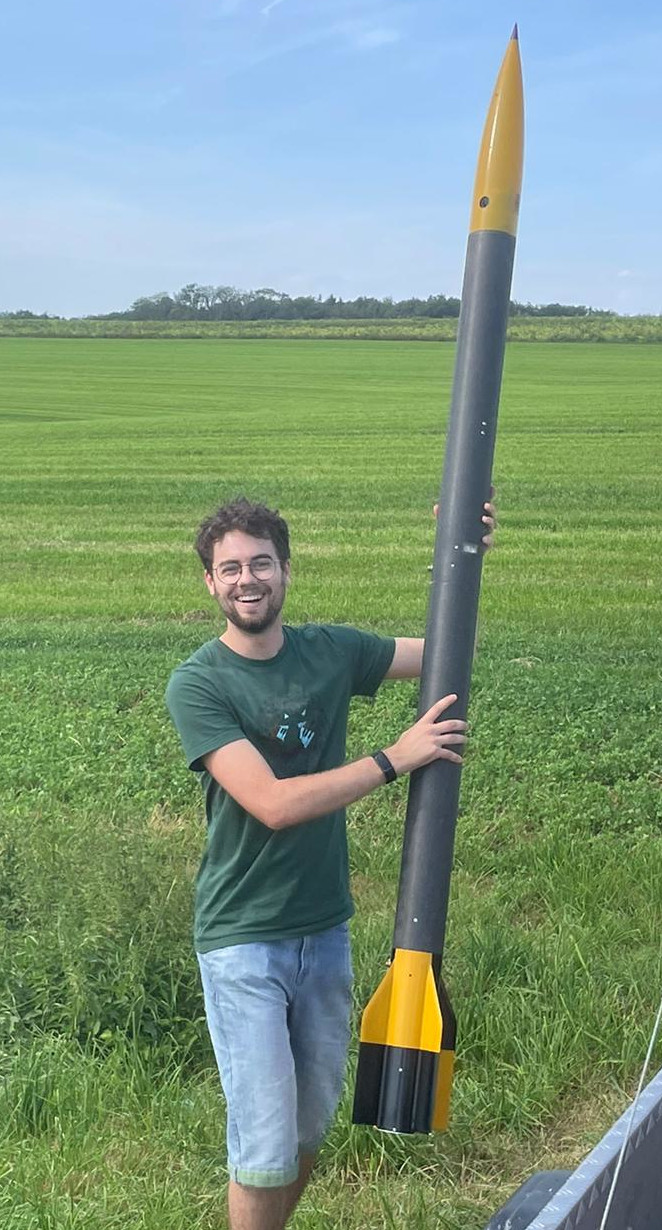
\includegraphics[width=\textwidth]{images/happy-jan.jpg}
  \column{0.65\textwidth}
  \begin{itemize}
    \item \href{mailto:jan.wolf@wuespace.de}{jan.wolf@wuespace.de} 
    \item Aerospace Computer Science since 2018 (MSc TBD)
    \item No electrical engineering background, all learning by doing
    \item WüSpace member since 2019
  \end{itemize}
  \end{columns}
\end{frame}

\begin{frame}{Who is this Nerd?}
  \begin{columns}
  \column{0.6\textwidth}
    Daedalus 2 Electronics
    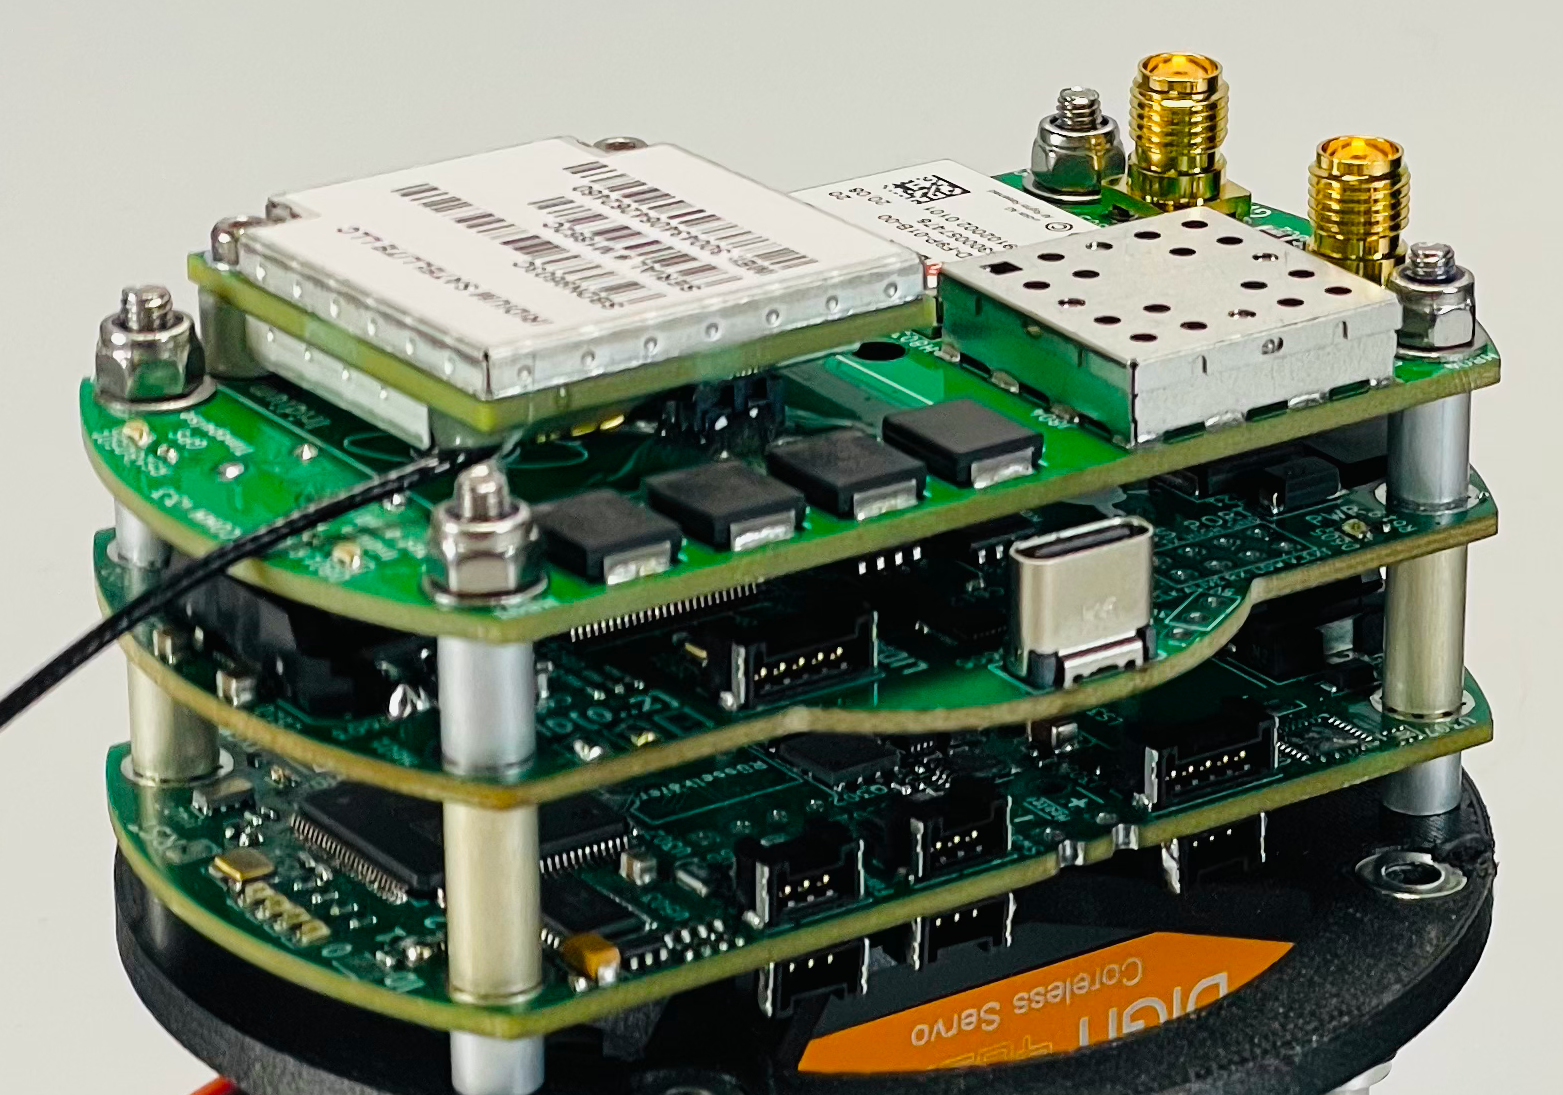
\includegraphics[width=\textwidth]{images/d2-pcb-stack.png}
  \column{0.4\textwidth}
  \pause
    \includegraphics[width=\textwidth]{images/d2-knüppel.jpg}\\
    BONK
    \vspace{1cm}

  \pause
    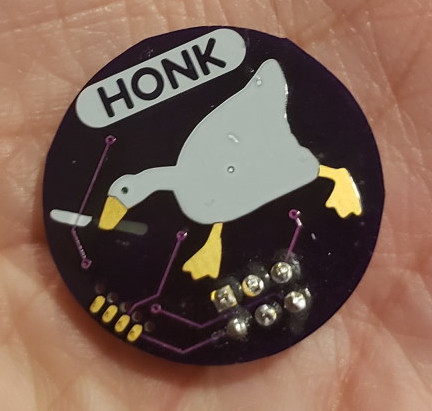
\includegraphics[width=0.6\textwidth]{images/honk.jpg}
    HONK
  \end{columns}
\end{frame}

\begin{frame}{Motivation}
  Why am I doing this?\\
  \pause
  \vspace{1cm}
  \begin{center}
  Because this guy kept bugging me about it\\
  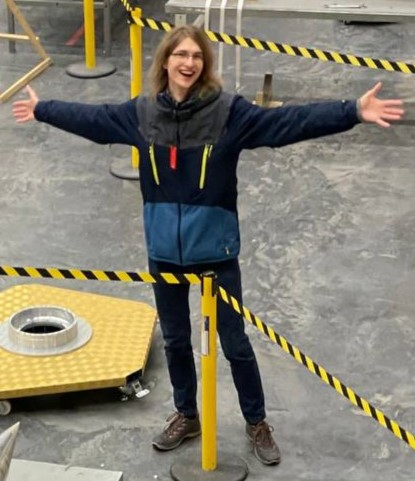
\includegraphics[width=0.8\textwidth]{images/philip.jpg}
  \end{center}
\end{frame}

\begin{frame}{Goal of this Course}
  What we'll do:
  \begin{itemize}
    \item Transfer of knowledge! Teach people how to design their own PCBs
    \item Learning by doing! Everybody will go through the process of designing a PCB
  \end{itemize}
  What we won't do:
  \begin{itemize}
    \item Teach how electronics work in general\\
    \pause Read a book or smth idk
  \end{itemize}
\end{frame}

\begin{frame}{Based on HOPE}
  \centering
  This course is \sout{stolen from} loosely based on the Hands-On PCB Engineering (HOPE) course from Berkeley. Take a look at their program, it's great! \href{https://ieee.berkeley.edu/hope/}{ieee.berkeley.edu/hope/}\\
  \vspace{1cm}
  
\includegraphics[width=0.8\textwidth]{images/HOPE-course.png}
\end{frame}

\section{What is a PCB?}
\subsection{PCB Examples}

\begin{frame}{Macbook Pro Logic Board}
  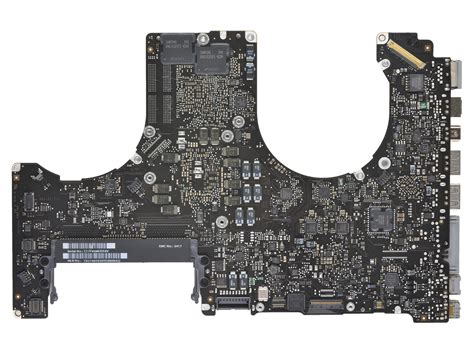
\includegraphics[width=\textwidth]{images/macbook.png}
\end{frame}

\begin{frame}{Starlink}
  \centering
  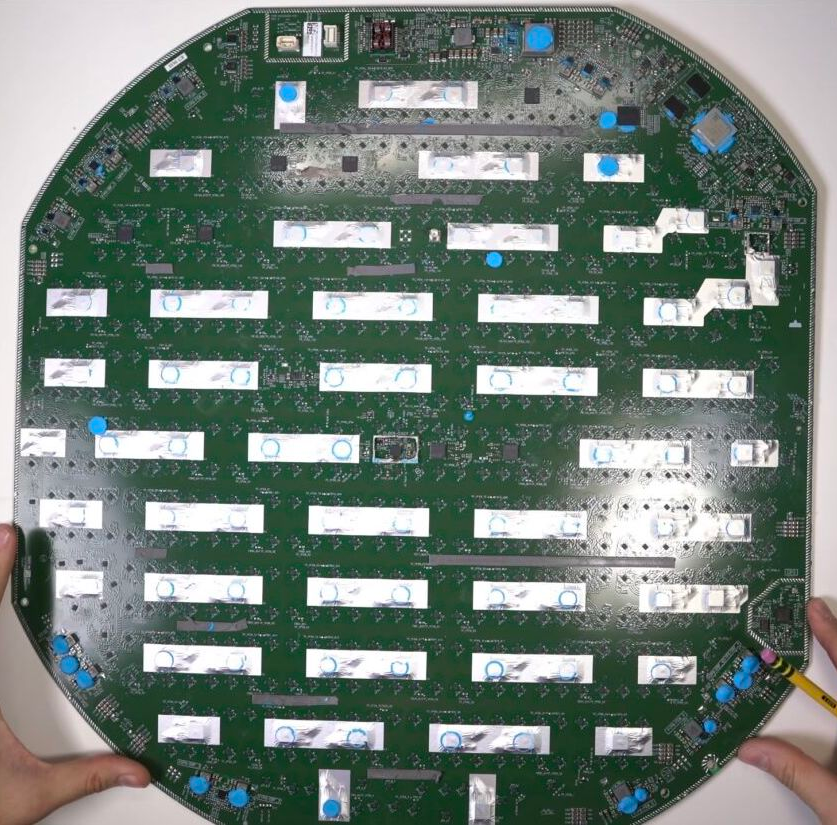
\includegraphics[width=0.45\textwidth]{images/starlink-pcb.png}
  \includegraphics[width=0.45\textwidth]{images/starlink-dish.png}
\end{frame}

\begin{frame}{And much more}
  \centering
  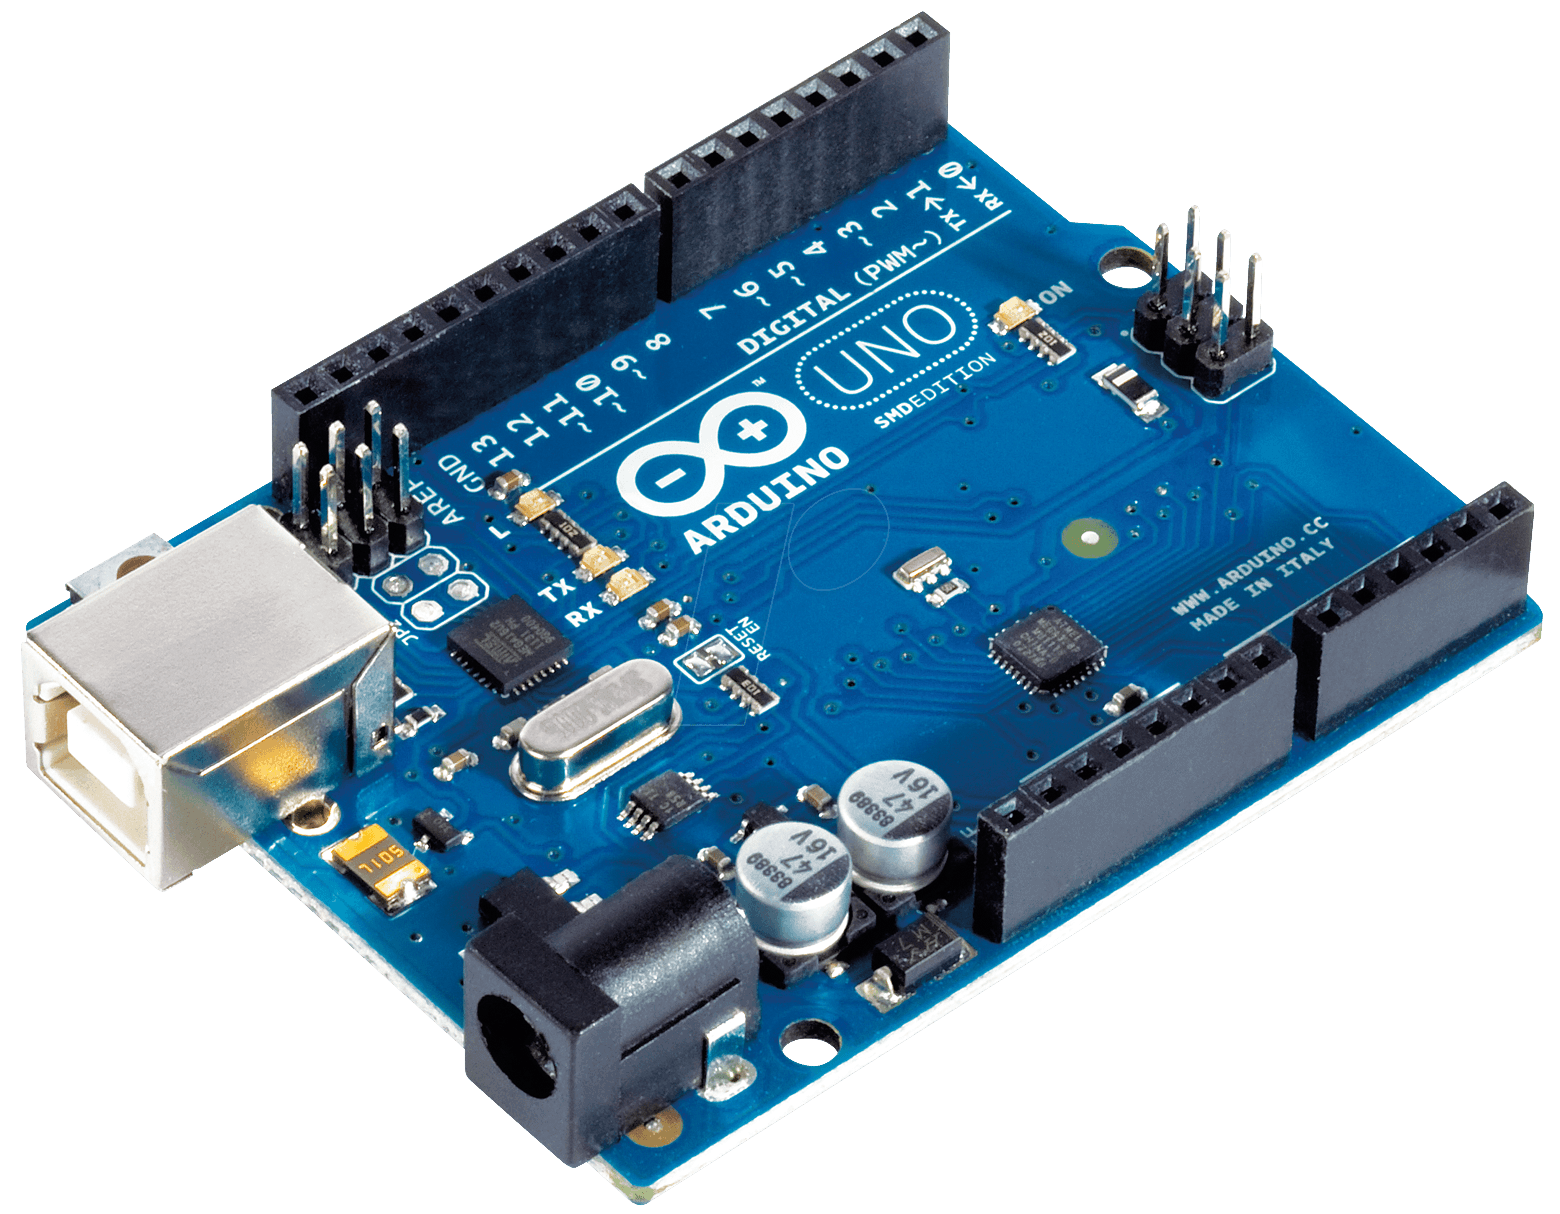
\includegraphics[width=0.35\textwidth]{images/arduino.png}
  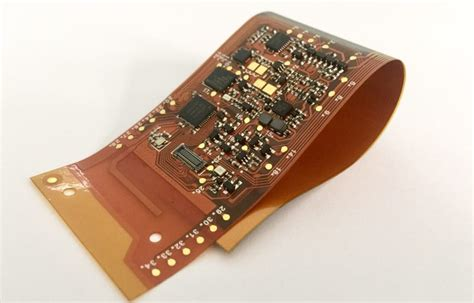
\includegraphics[width=0.55\textwidth]{images/flex-pcb.png}
  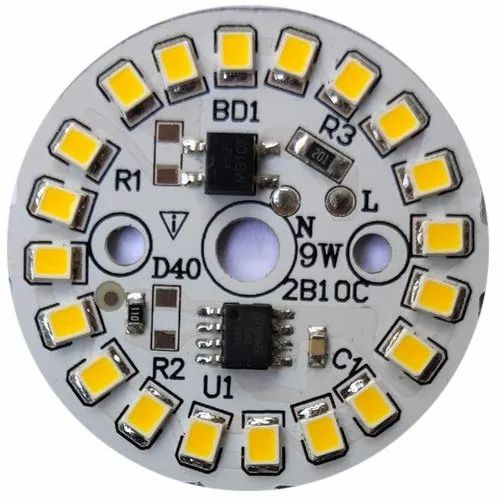
\includegraphics[width=0.25\textwidth]{images/led-pcb.png}
  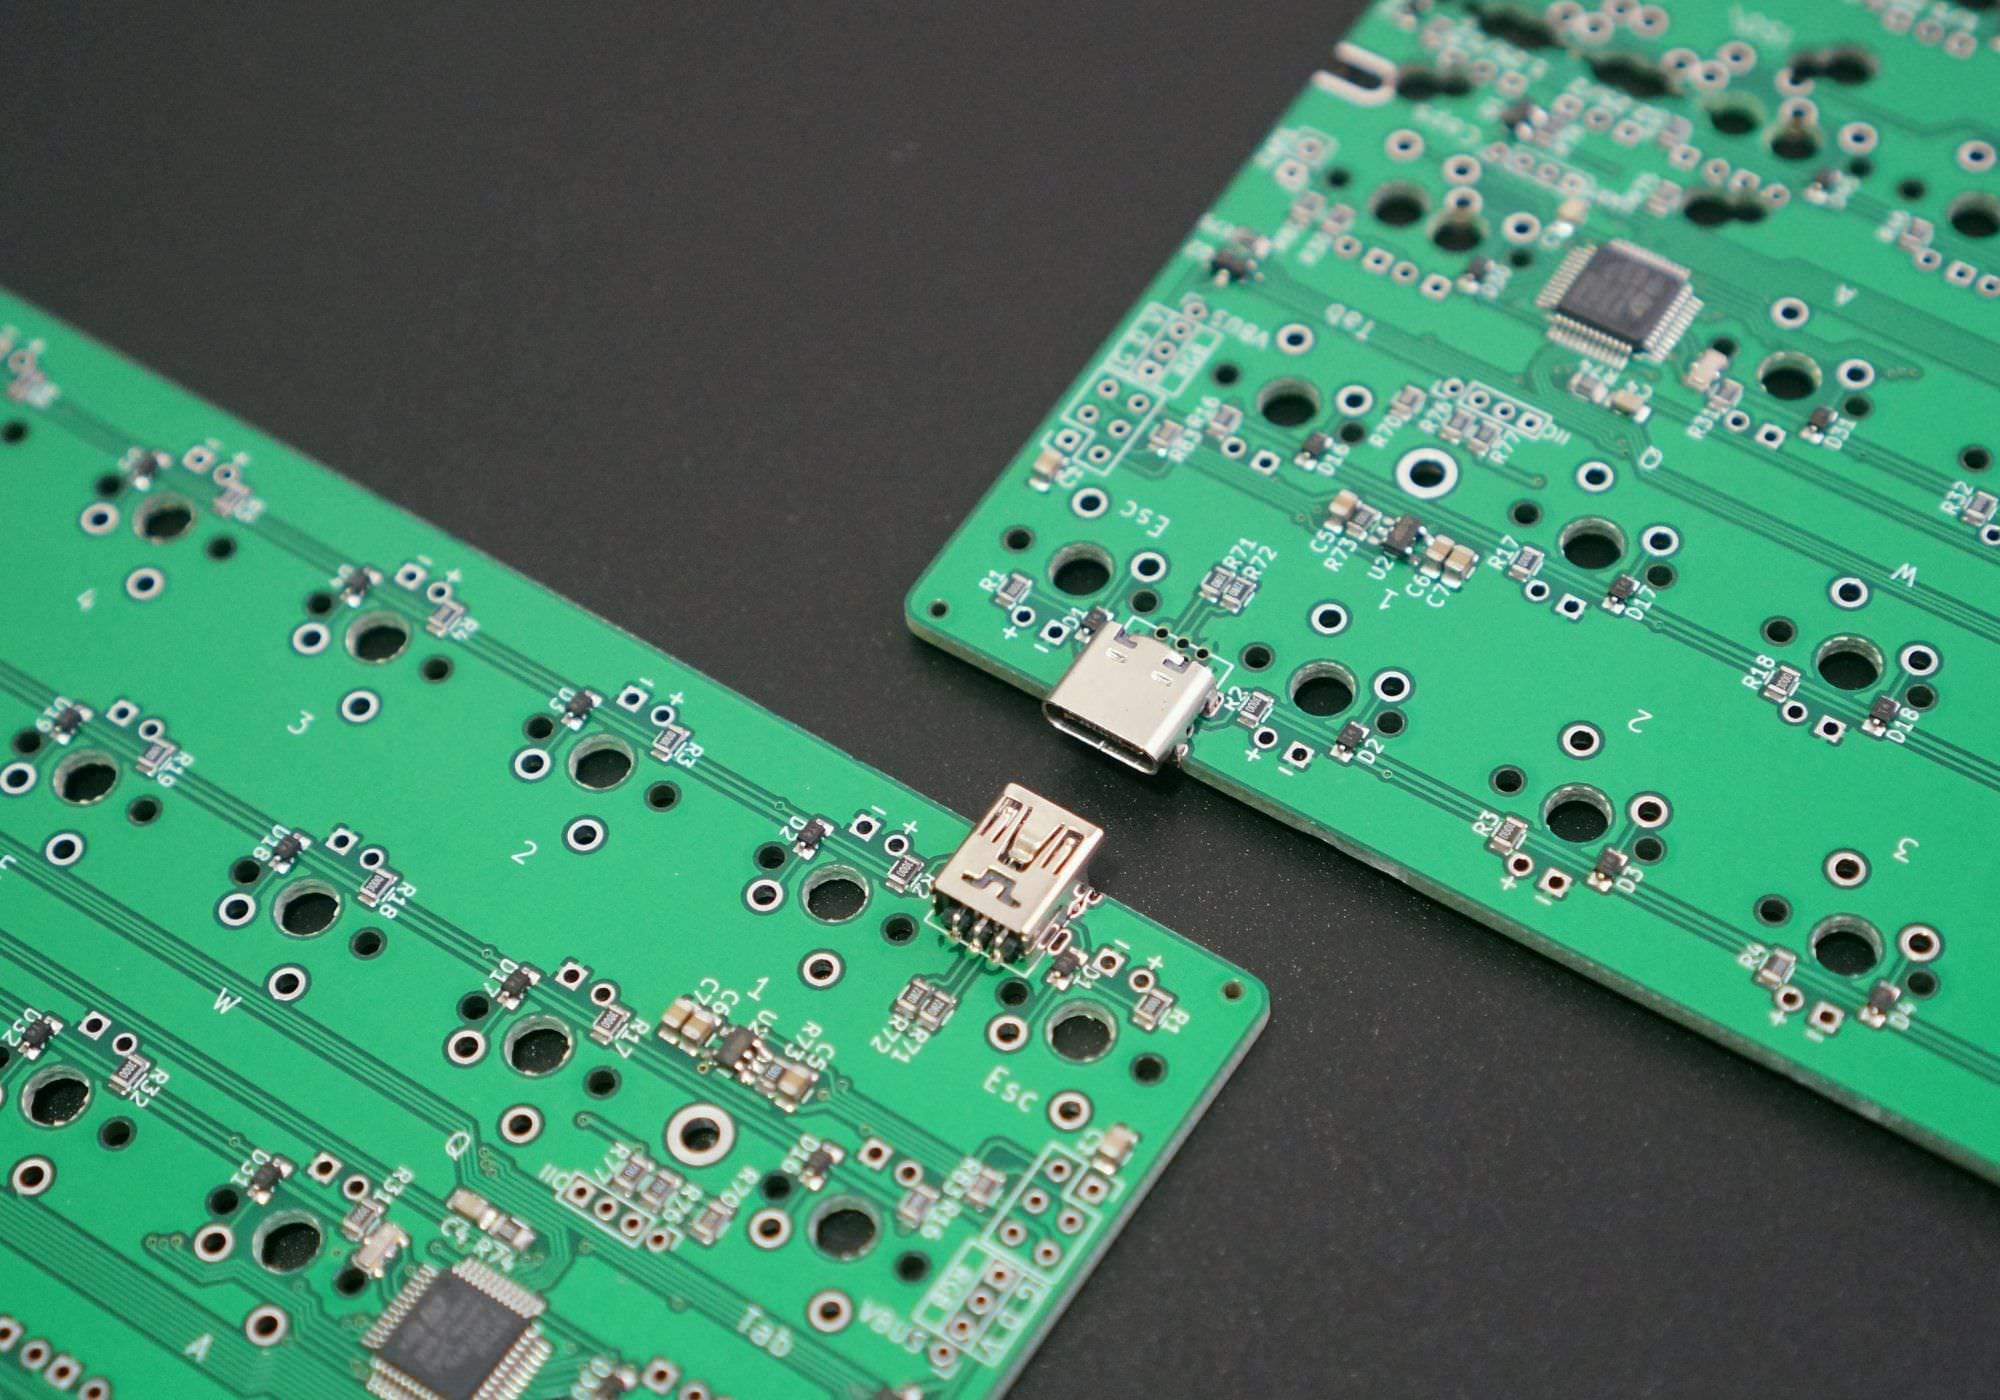
\includegraphics[width=0.45\textwidth]{images/keyboard-pcb.png}
\end{frame}

\subsection{PCB Construction}

\begin{frame}{What is a PCB?}
  \begin{itemize}
    \item PCBs (printed circuit board) are essential to electronic hardware design
    \item They provide form (mechanical) and function (electrical)
    \item Better, cheaper and more reliable than alternatives
  \end{itemize}
\end{frame}

\begin{frame}{What is a PCB?}
  \centering
  Sandwich of conductive layers!\\
  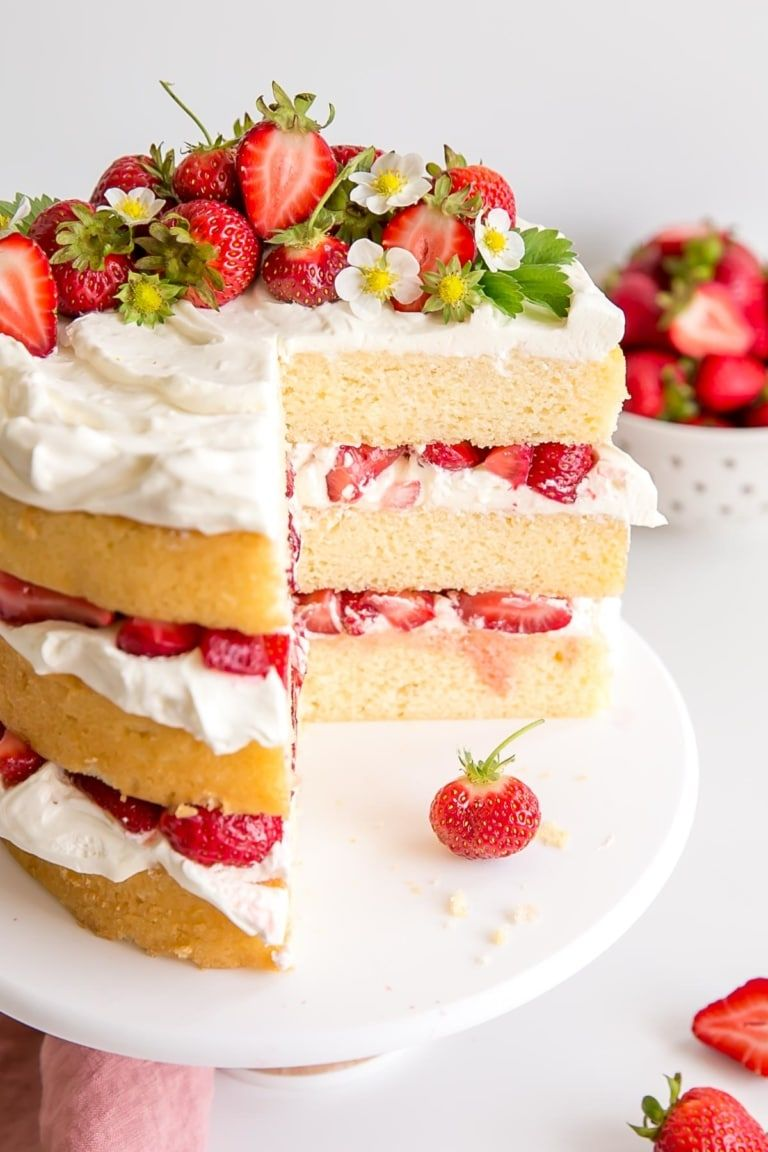
\includegraphics[width=0.3\textwidth]{images/cake-cross-section.png}
  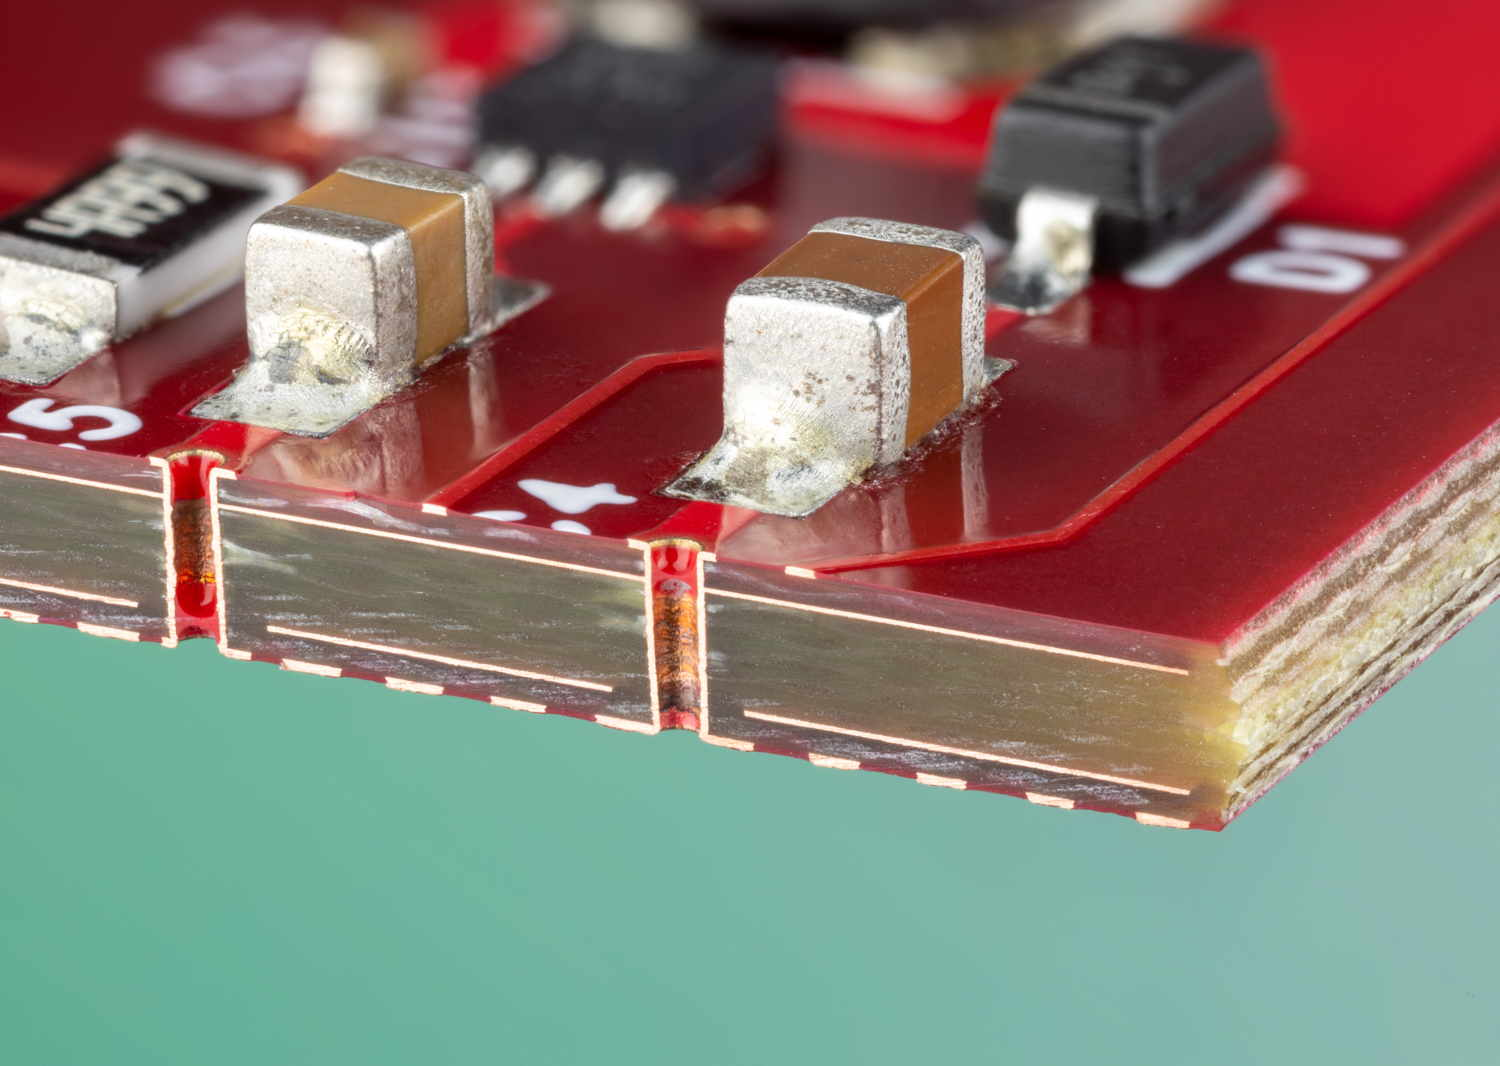
\includegraphics[width=0.6\textwidth]{images/pcb-cross-section.png}
\end{frame}

\begin{frame}{What is a PCB?}
  \centering
  More layers are possible (although expensive)
  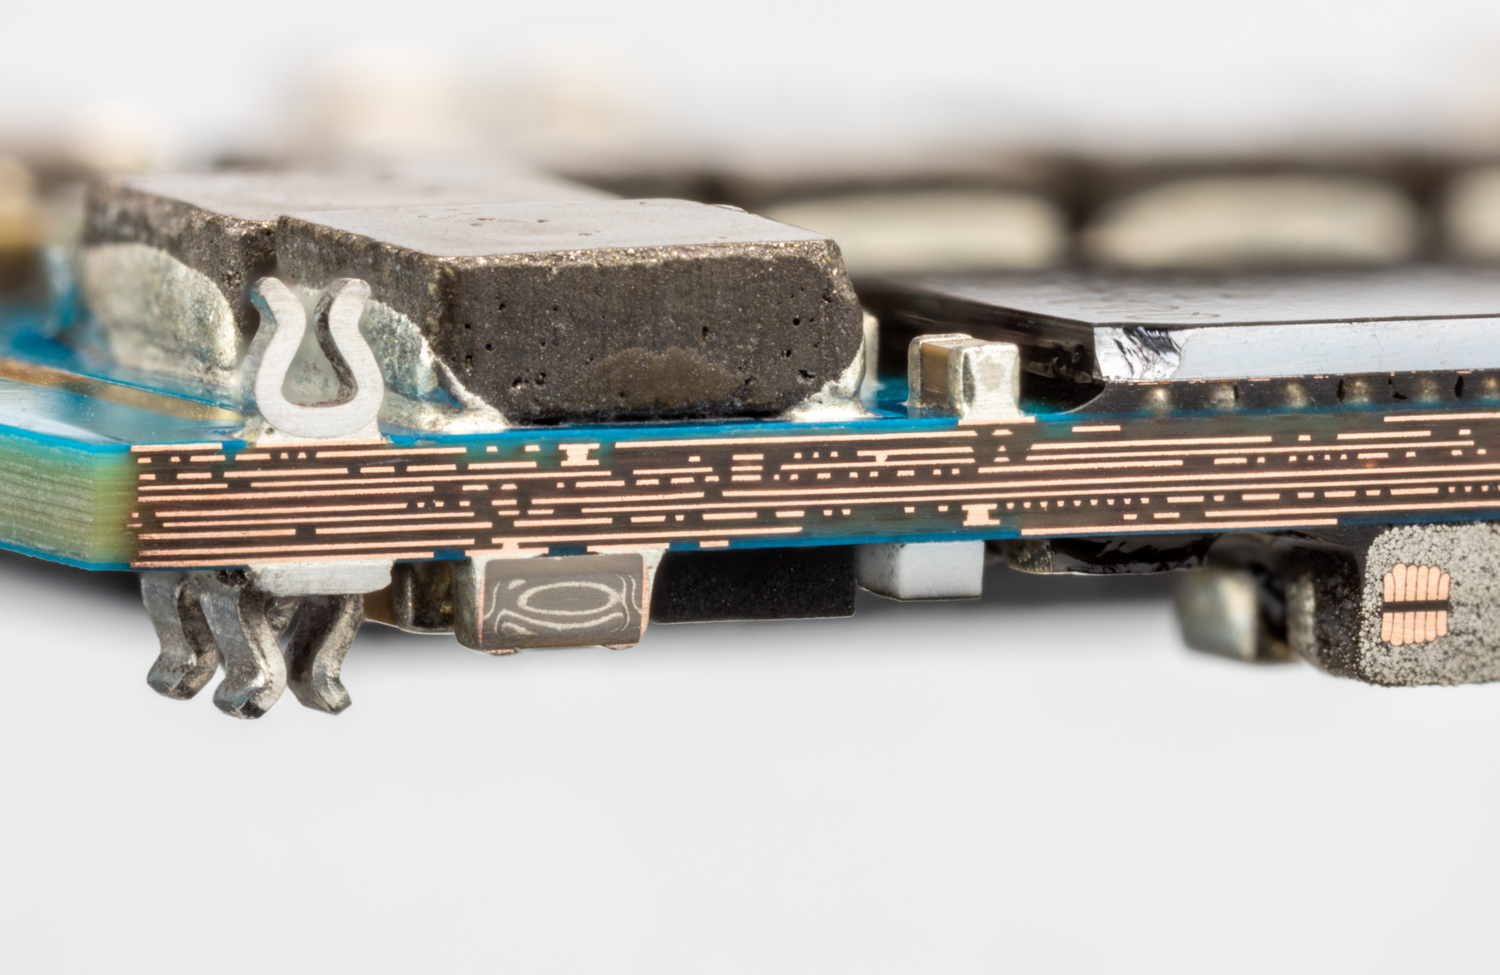
\includegraphics[width=\textwidth]{images/open-circuit2.jpg}\\
  Find more brilliant pictures at \href{https://www.opencircuitsbook.com/}{www.opencircuitsbook.com/}
\end{frame}

\subsection{PCB Features}

\begin{frame}{PCB Features}
  \begin{itemize}
    \item \textbf{Tracks/Traces} are basically wires between components
    \item \textbf{Pads} make electrical connection to components, fat copper areas.
    \item \textbf{Vias} are holes with conductive plating to jump between layers
  \end{itemize}
\end{frame}

\begin{frame}{THT Components}
  Components can be THT (through hole technology)...\\
  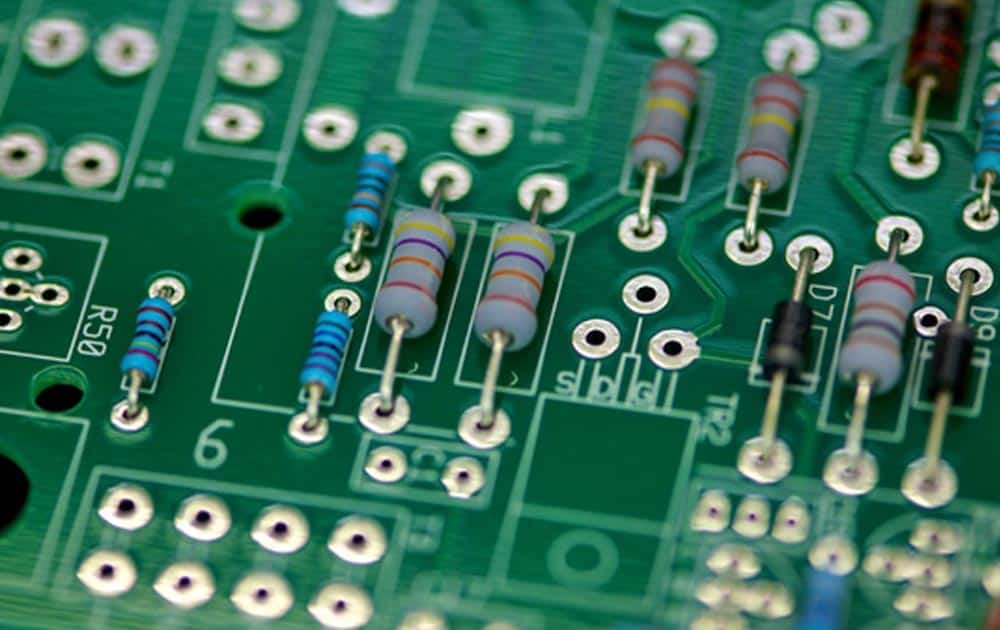
\includegraphics[width=\textwidth]{images/tht-placement.png}
\end{frame}

\begin{frame}{SMD Components}
  or SMD (surface mount devices)\\
  \begin{center}
    \includegraphics[width=0.8\textwidth]{images/smd-placement.png}
  \end{center}
\end{frame}


\section{PCB Design Tools}

\subsection{Available ECAD Tools}

\begin{frame}{Terminology}
  EDA = ECAD\\
  Electronic Design Automation\\
  Electronic Computer Aided Design\\
  \pause
  \vspace{1cm}
  ...how to pronounce KiCad?\\
  \pause
  
\includegraphics[width=0.8\textwidth]{images/kicad-pronounce.jpg}
\end{frame}

\begin{frame}{Other ECAD Programs are Available}
  
\includegraphics[width=\textwidth]{images/ecad-logos.png}
  \pause
  Some of these can simulate Maxwall's equation, design 20 layer PCBs and cost 40k€/year.\\
  \pause
  Others are basically MS Paint in a trench coat.
\end{frame}

\subsection{KiCad!}

\begin{frame}{KiCad}
  \begin{center}
    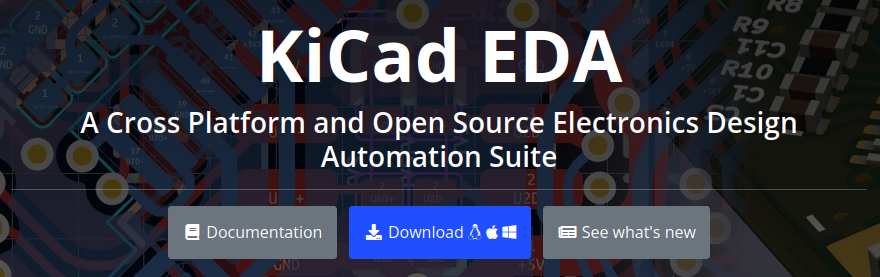
\includegraphics[width=\textwidth]{images/kicad-banner.png}
  \end{center}
  \vspace{-0.2cm}
  \begin{itemize}
    \item Free and Open Source (GPLv3)
    \item Windows, Mac, Linux, BSD compatible
    \item Released at ITU Grenoble 1992, receives funding by CERN, part of the Linux Foundation
    \item Easy file formats and open APIs: Lots of compatibility, 3rd party plugins and libraries
  \end{itemize}
\end{frame}

\begin{frame}{KiCad Community}
  \centering
  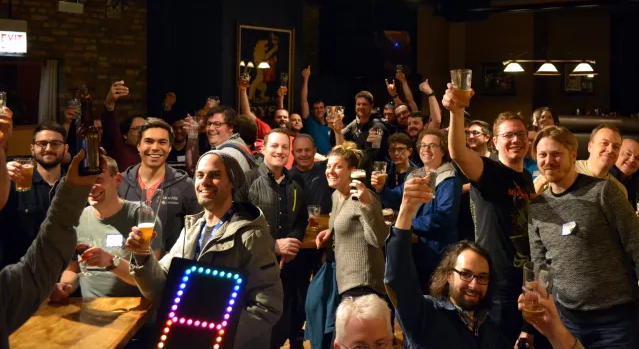
\includegraphics[width=0.6\textwidth]{images/kicon-crowded.png}
  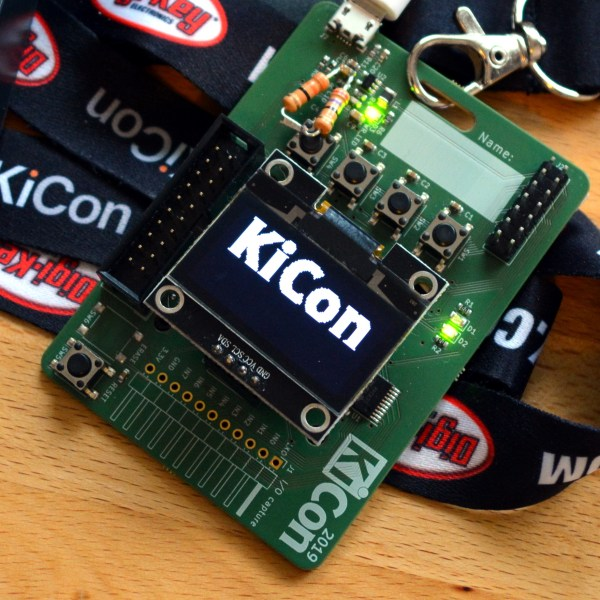
\includegraphics[width=0.25\textwidth]{images/kicon.jpg}
  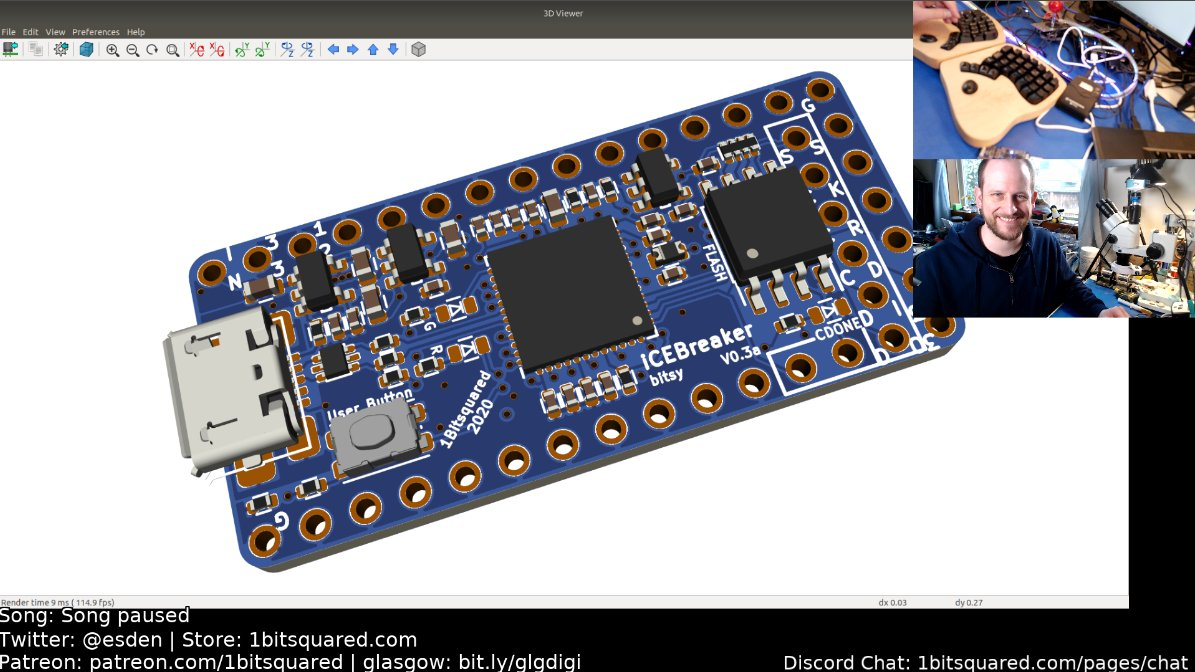
\includegraphics[width=0.45\textwidth]{images/kicad-live.jpg}
  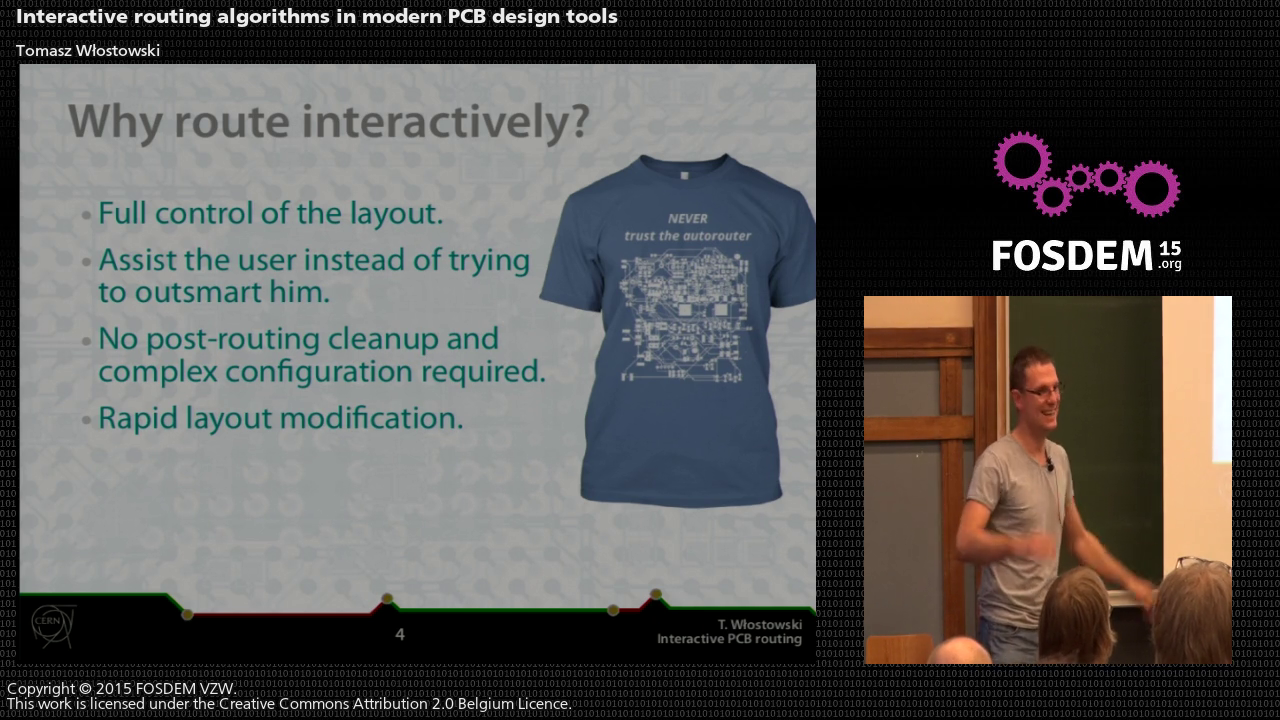
\includegraphics[width=0.45\textwidth]{images/kicad-fosdem.png}
  Nerdy hackers and makers available on Hackaday/Social Media/Livestreams/Conferences...
%  Twitter\tiny, formerly known as X, formerly known as Twitter
\end{frame}

\subsection{PCB Design Flow}

\begin{frame}{PCB Project Design Flow}
  \centering
  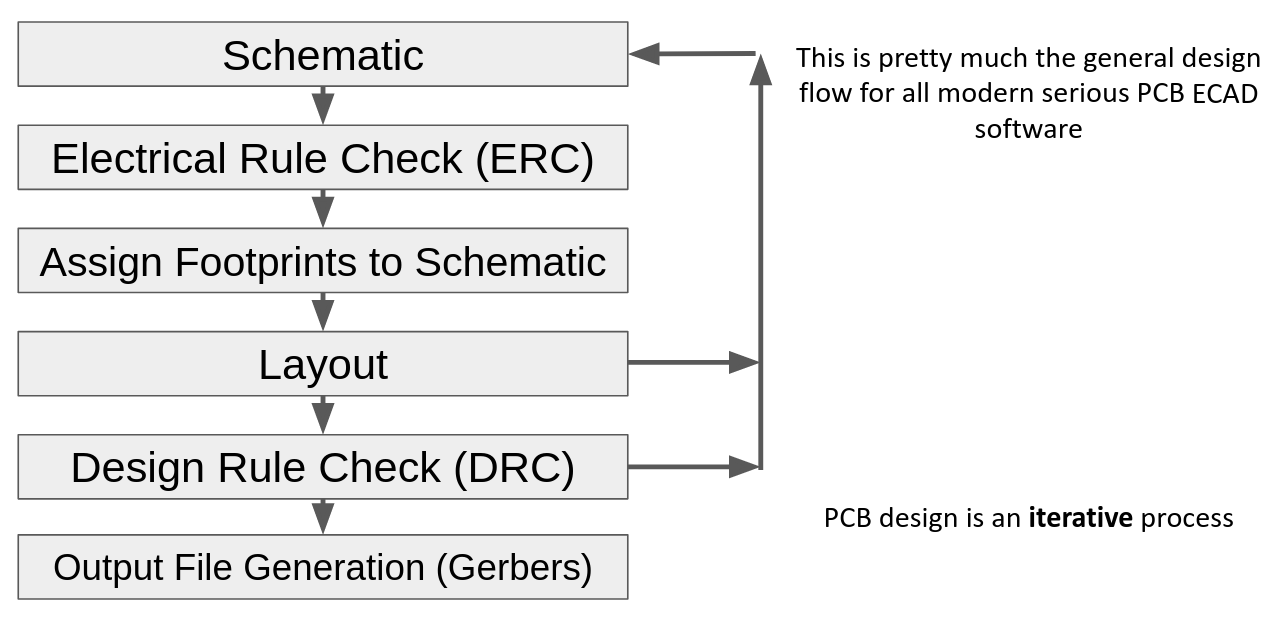
\includegraphics[width=\textwidth]{images/design-flow.png} 
\end{frame}

\begin{frame}{PCB Project Design Flow}
  \centering
  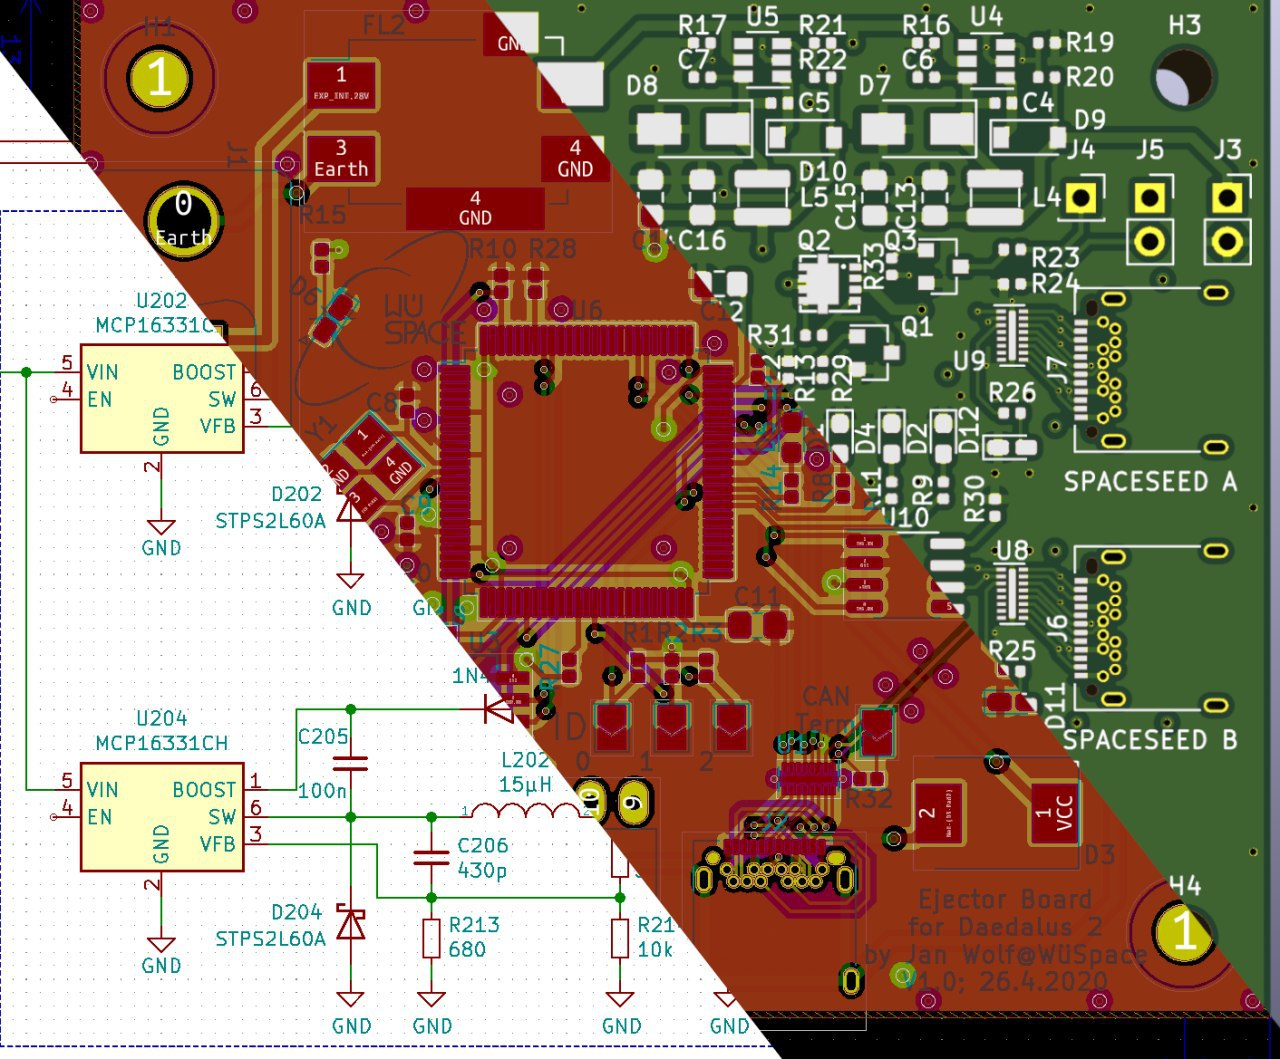
\includegraphics[width=0.8\textwidth]{images/kicad-process.jpg}
\end{frame}

\begin{frame}{PCB Project Design Flow}
  \centering
  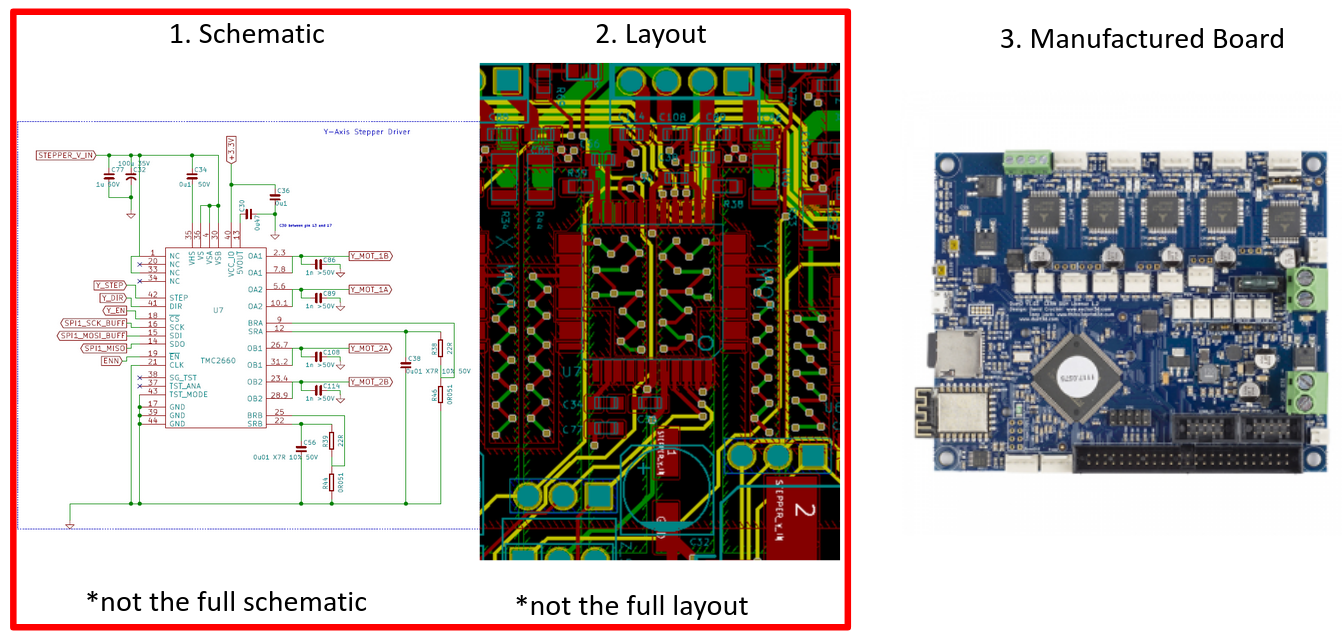
\includegraphics[width=\textwidth]{images/design-flow2.png}
\end{frame}

\section{Schematics}
\subsection{Schematic Flow}

\begin{frame}{Schematic Flow}
  Draw schematic
  \begin{itemize}
    \item Describe the circuit in a way both humans and computers understand
    \item ERC (electrical rule check) can catch errors
    \item Assign footprints 
  \end{itemize}
\end{frame}

\begin{frame}{Component Symbols}
  \begin{columns}
    \column{0.6\textwidth}
    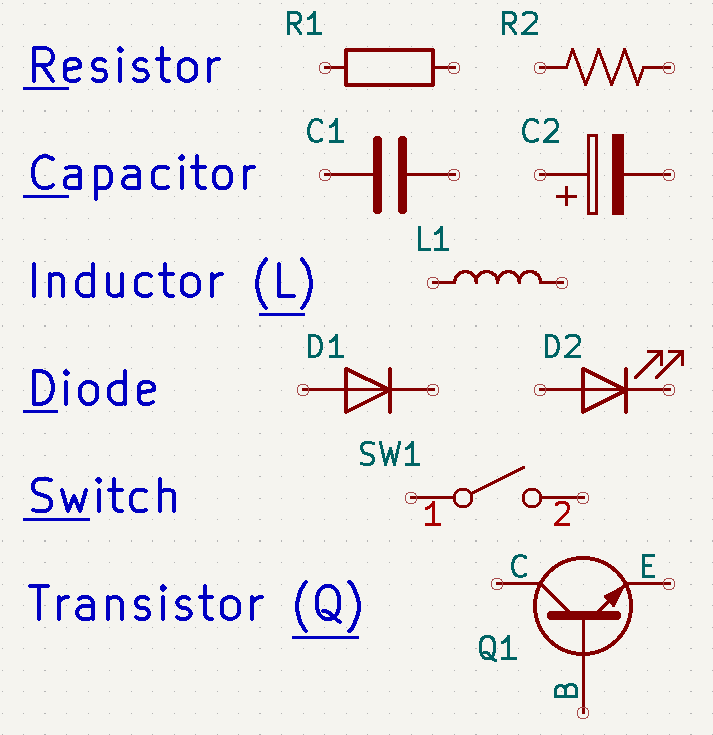
\includegraphics[width=\textwidth]{images/component-alphabet.png}
    \column{0.4\textwidth}
    Circuits are built from a few basic components, which follow a symbol ``alphabet''.\\

    Do you know any more non-IC components?
  \end{columns}
\end{frame}

\begin{frame}{Schematic Flow}
  \centering
  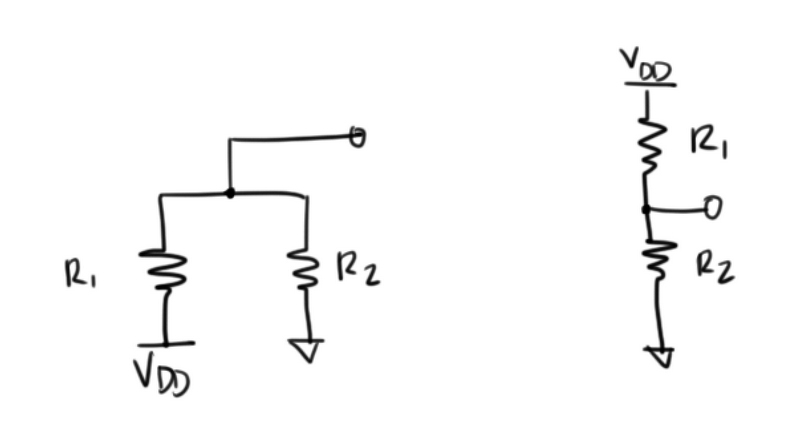
\includegraphics[width=0.8\textwidth]{images/voltage-div-orient.png}\\
  What does this do? Which one do you prefer?
\end{frame}

\begin{frame}{Schematic Flow}
  \centering
  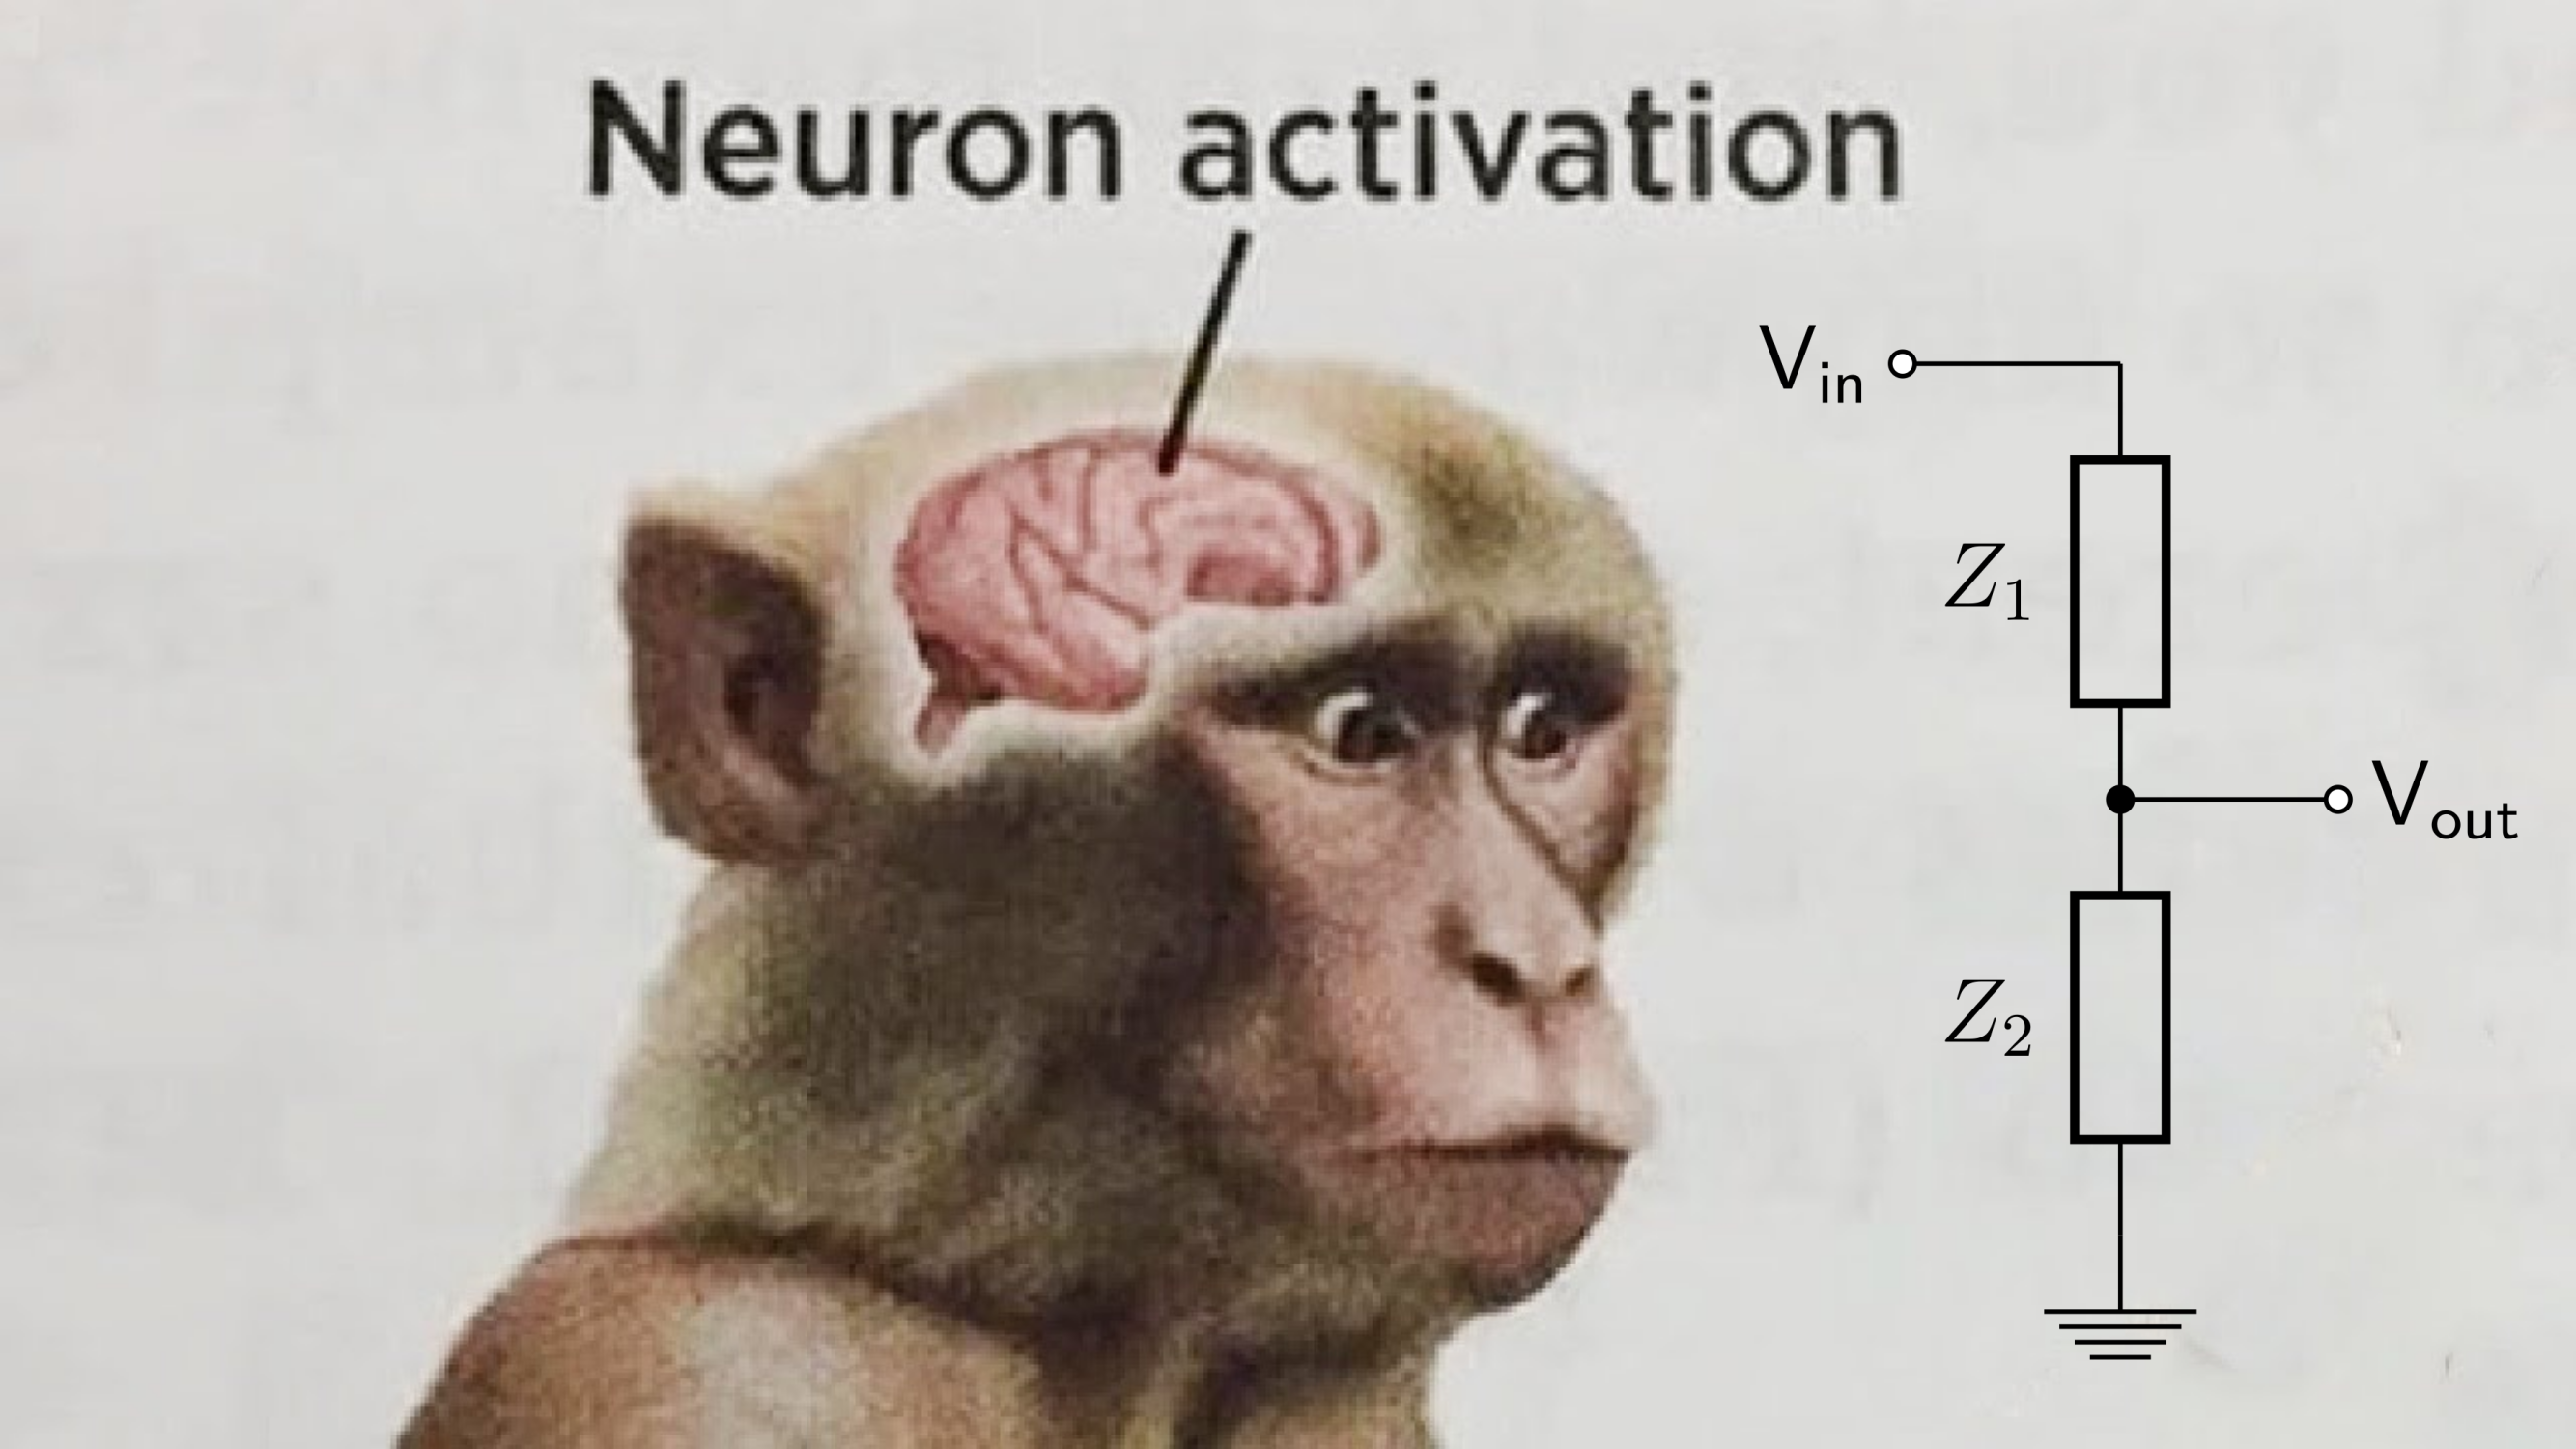
\includegraphics[width=\textwidth]{images/neuron-activation.png}
  \vspace{1cm}
  Following conventions makes understanding easier!
\end{frame}

\begin{frame}{Schematic Flow}
  Try to follow this general pattern:\\
  \vspace{0.2cm}
  \centering
  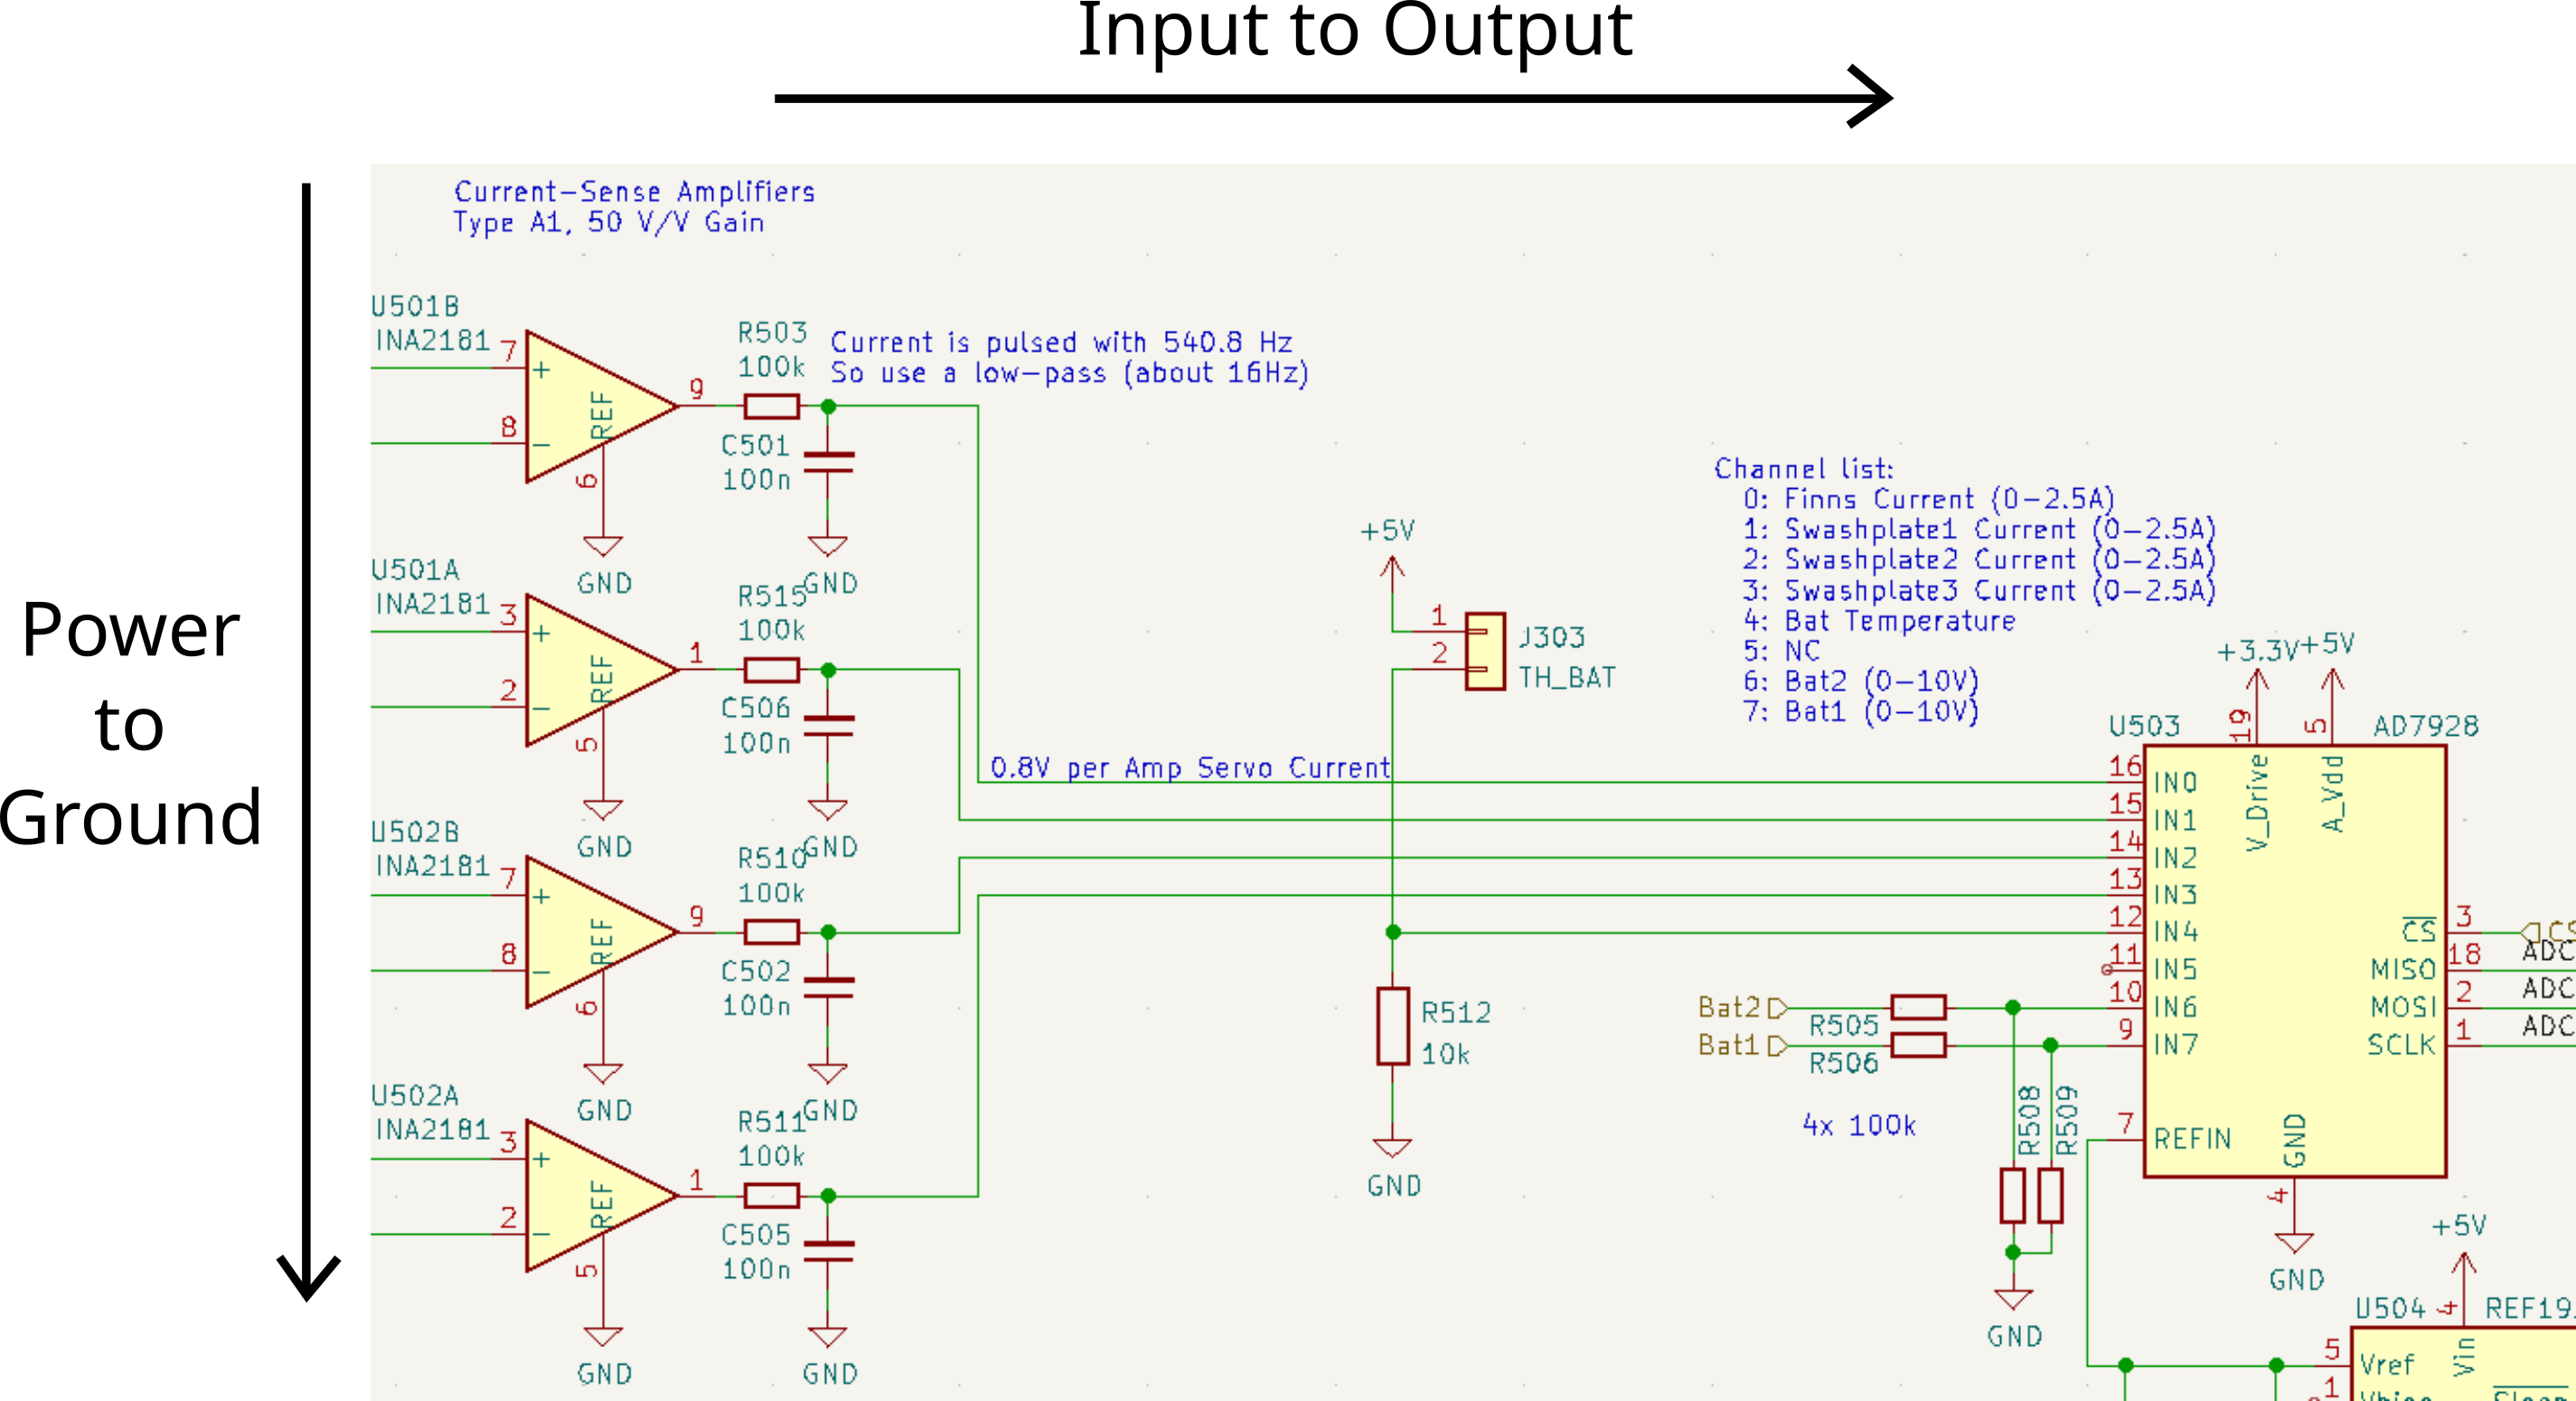
\includegraphics[width=\textwidth]{images/general-flow.png} 
  \pause
  (not always possible)
\end{frame}

\begin{frame}{Schematic Flow}
  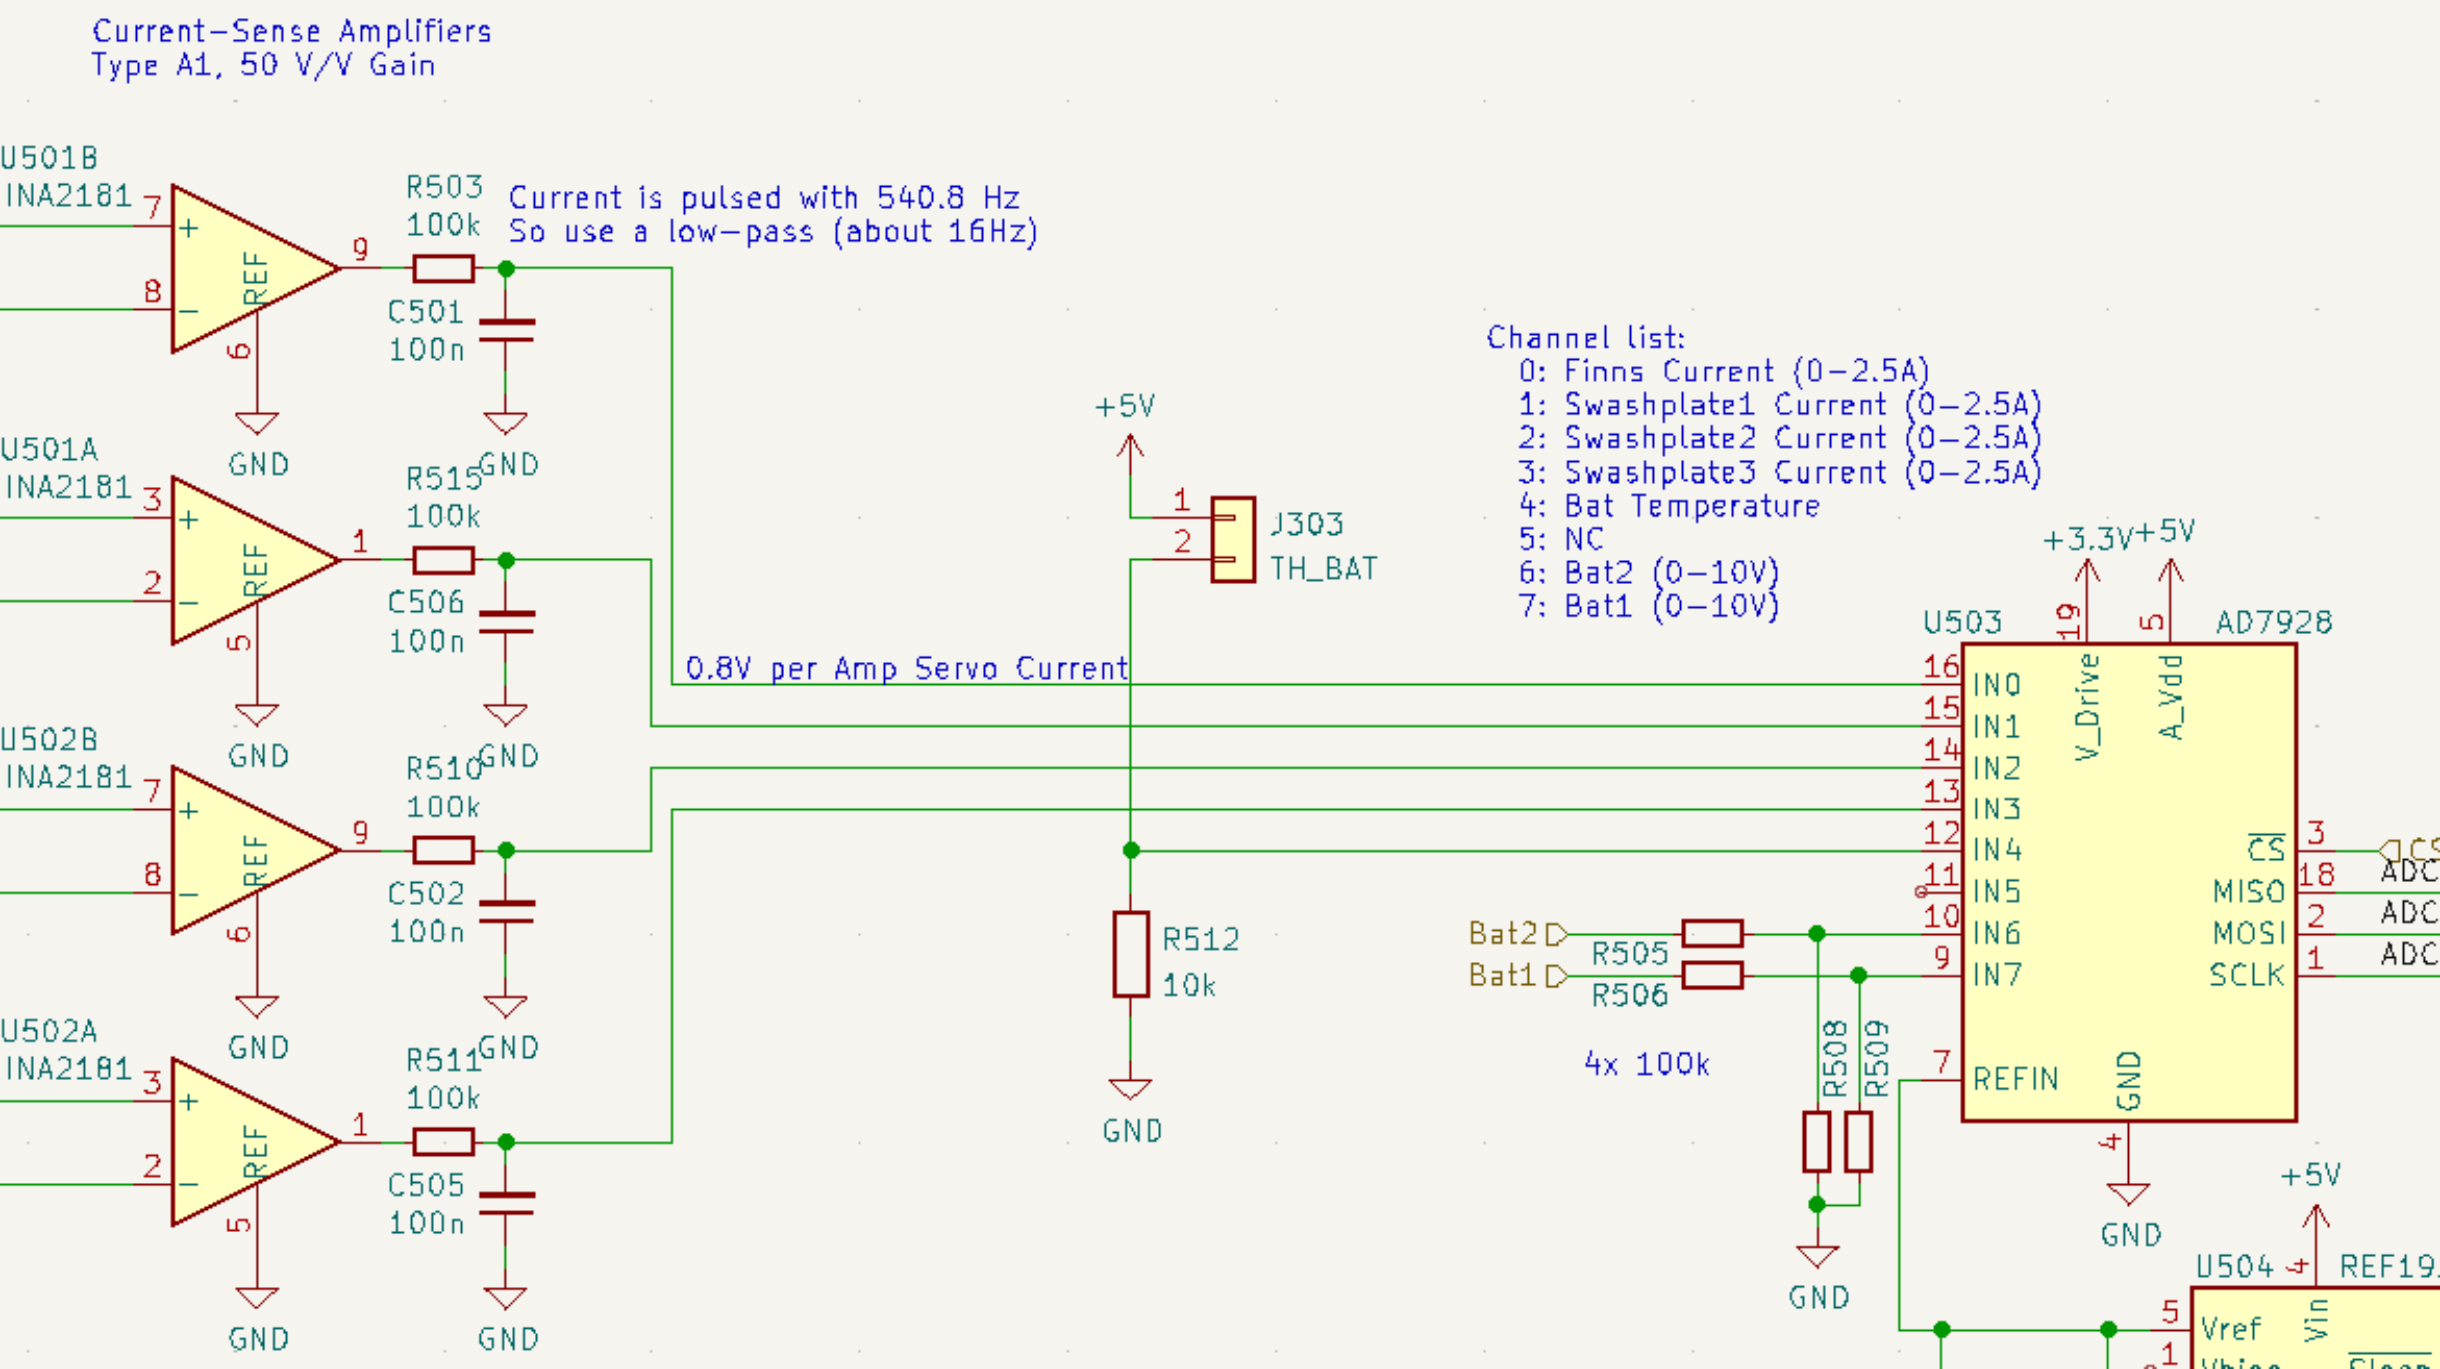
\includegraphics[width=\textwidth]{images/ex1.png} 
\end{frame}

\begin{frame}{Schematic Flow}
  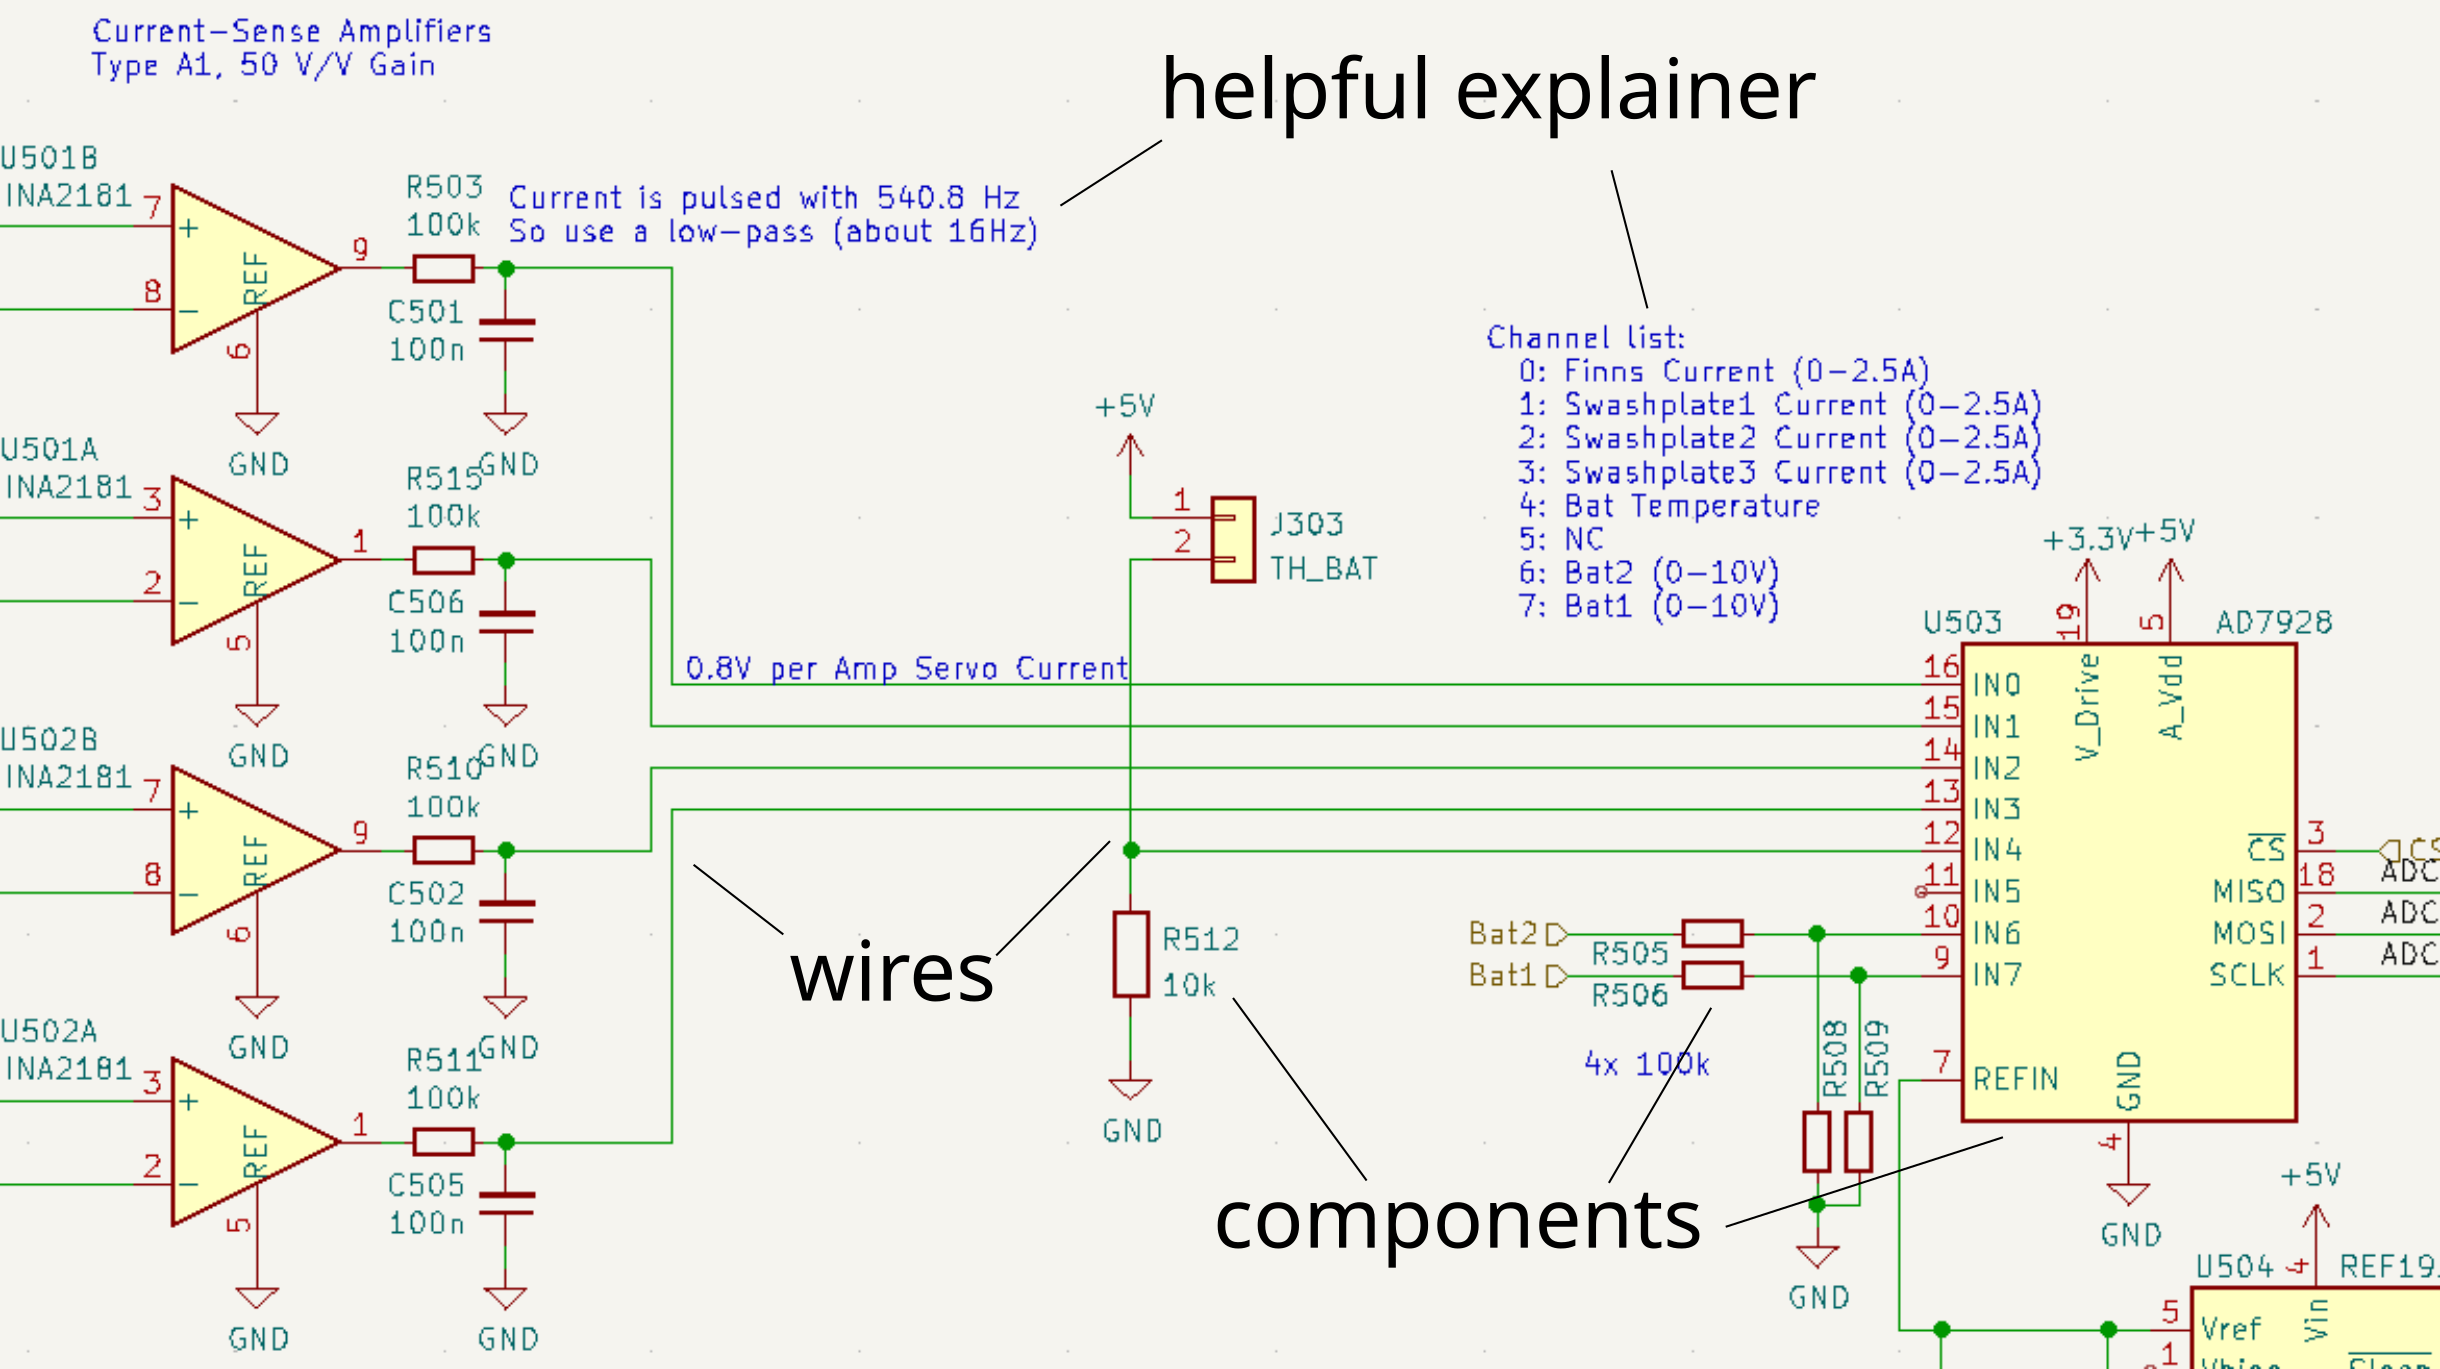
\includegraphics[width=\textwidth]{images/ex1-1.png} 
\end{frame}

\begin{frame}{Schematic Flow}
  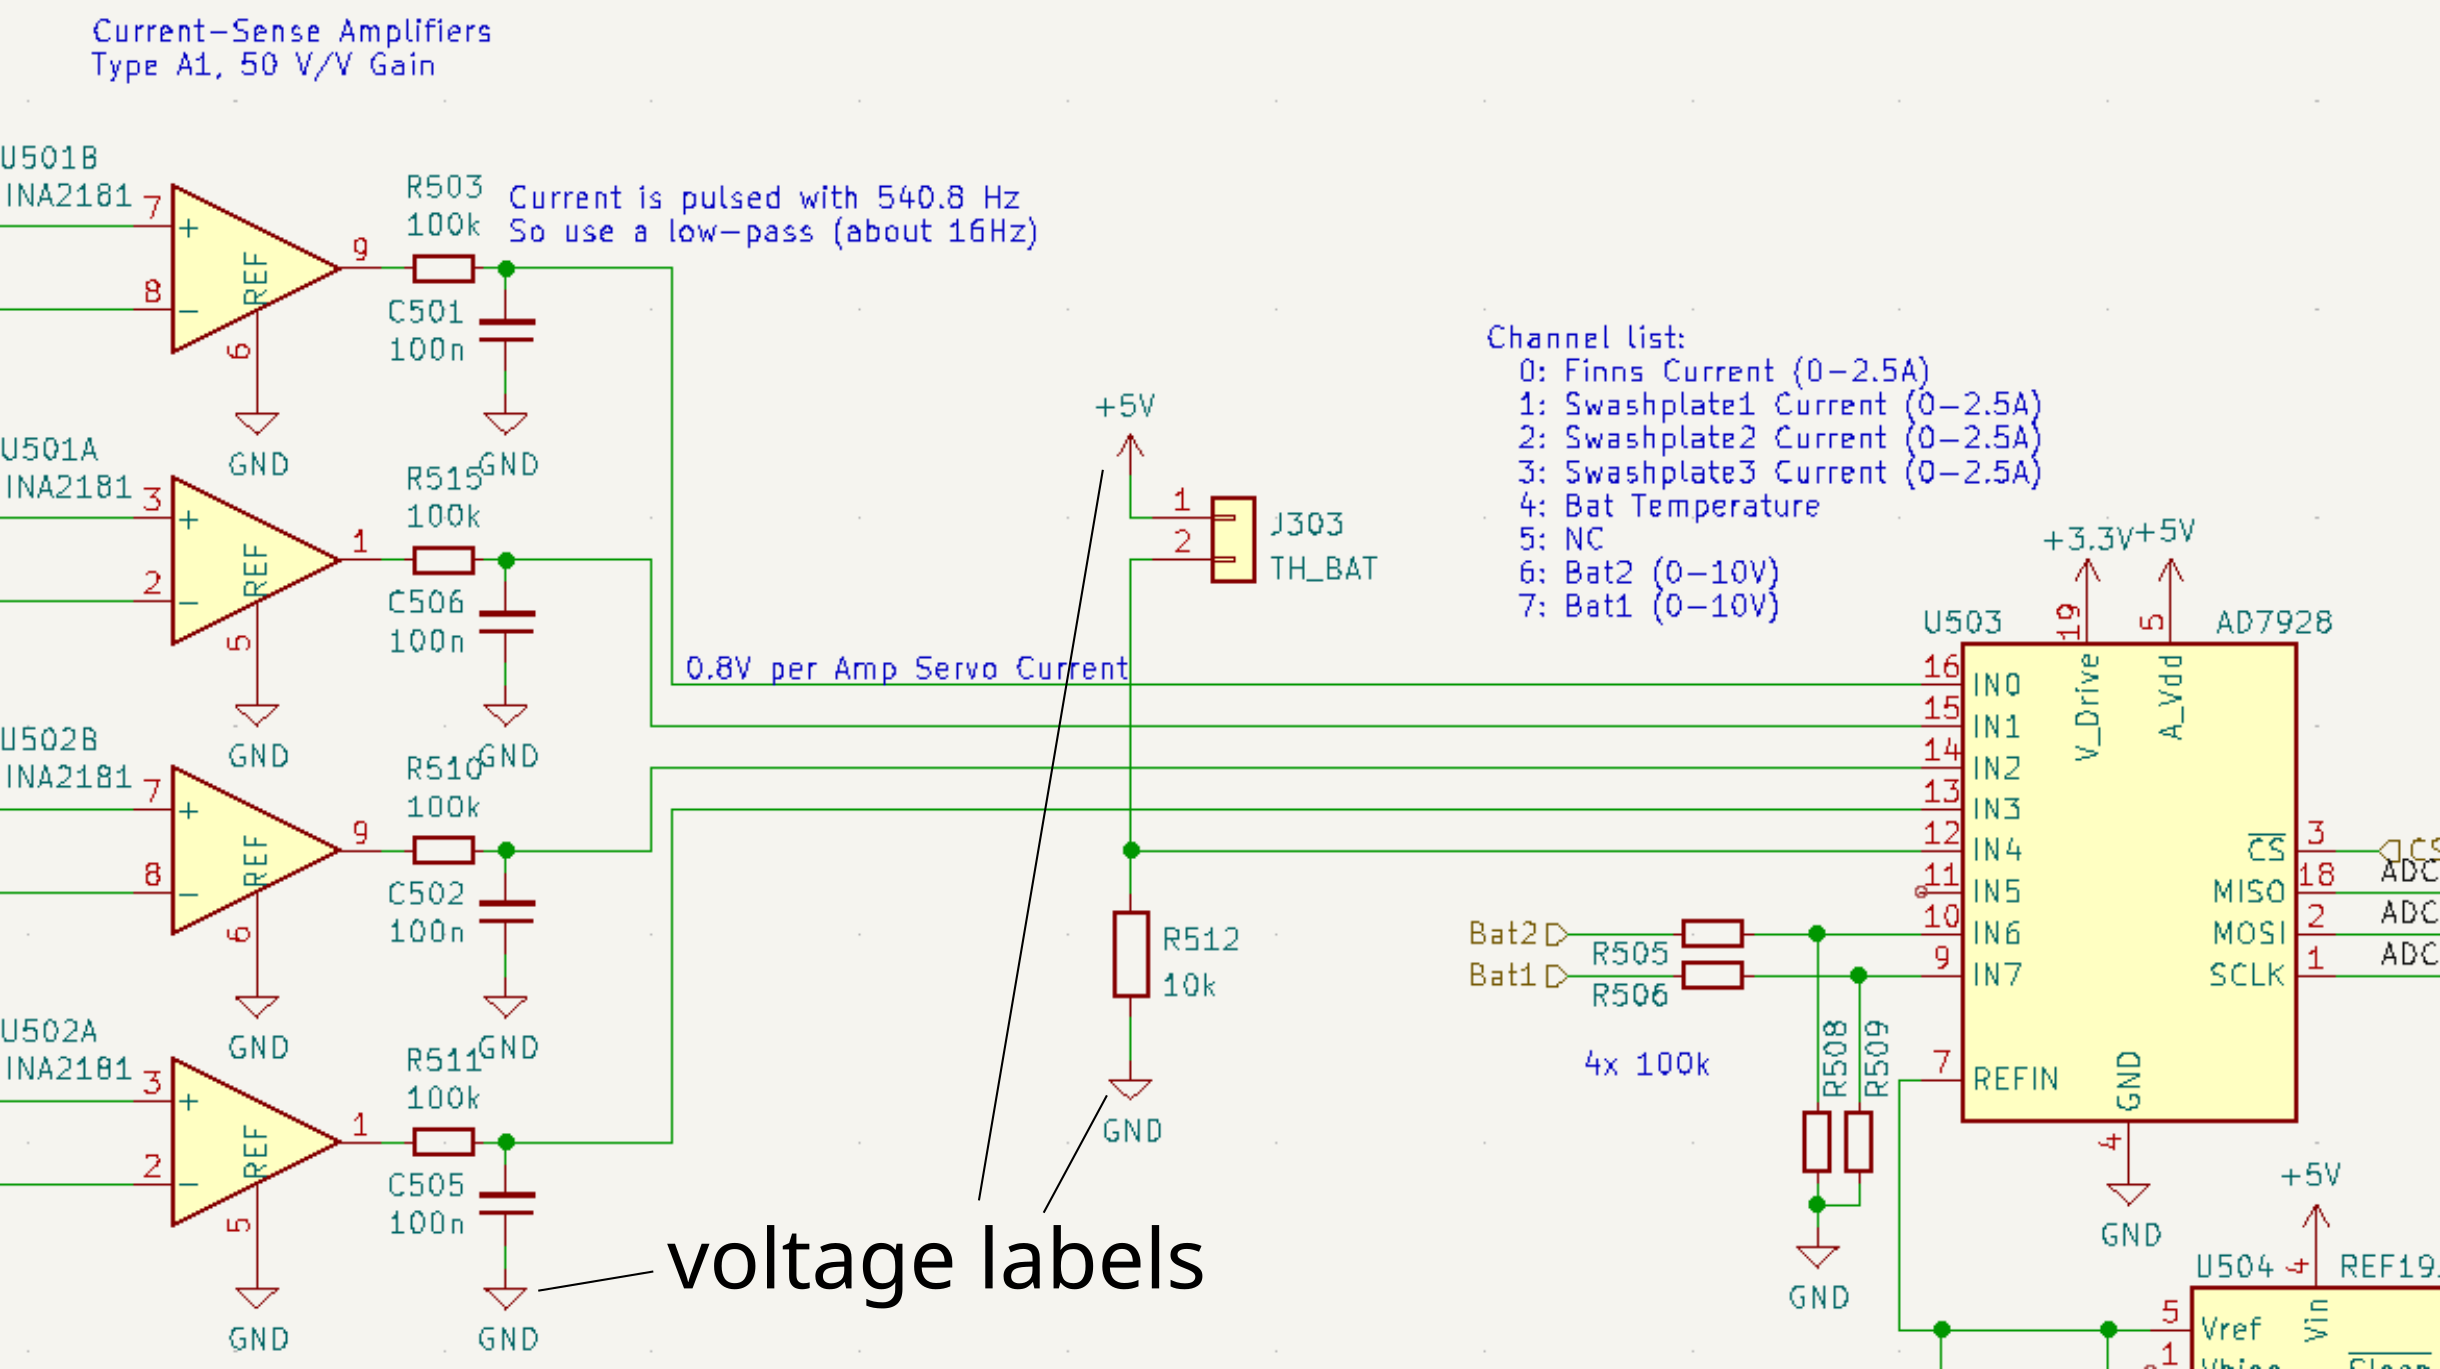
\includegraphics[width=\textwidth]{images/ex1-2.png} 
\end{frame}

\begin{frame}{Schematic Flow}
  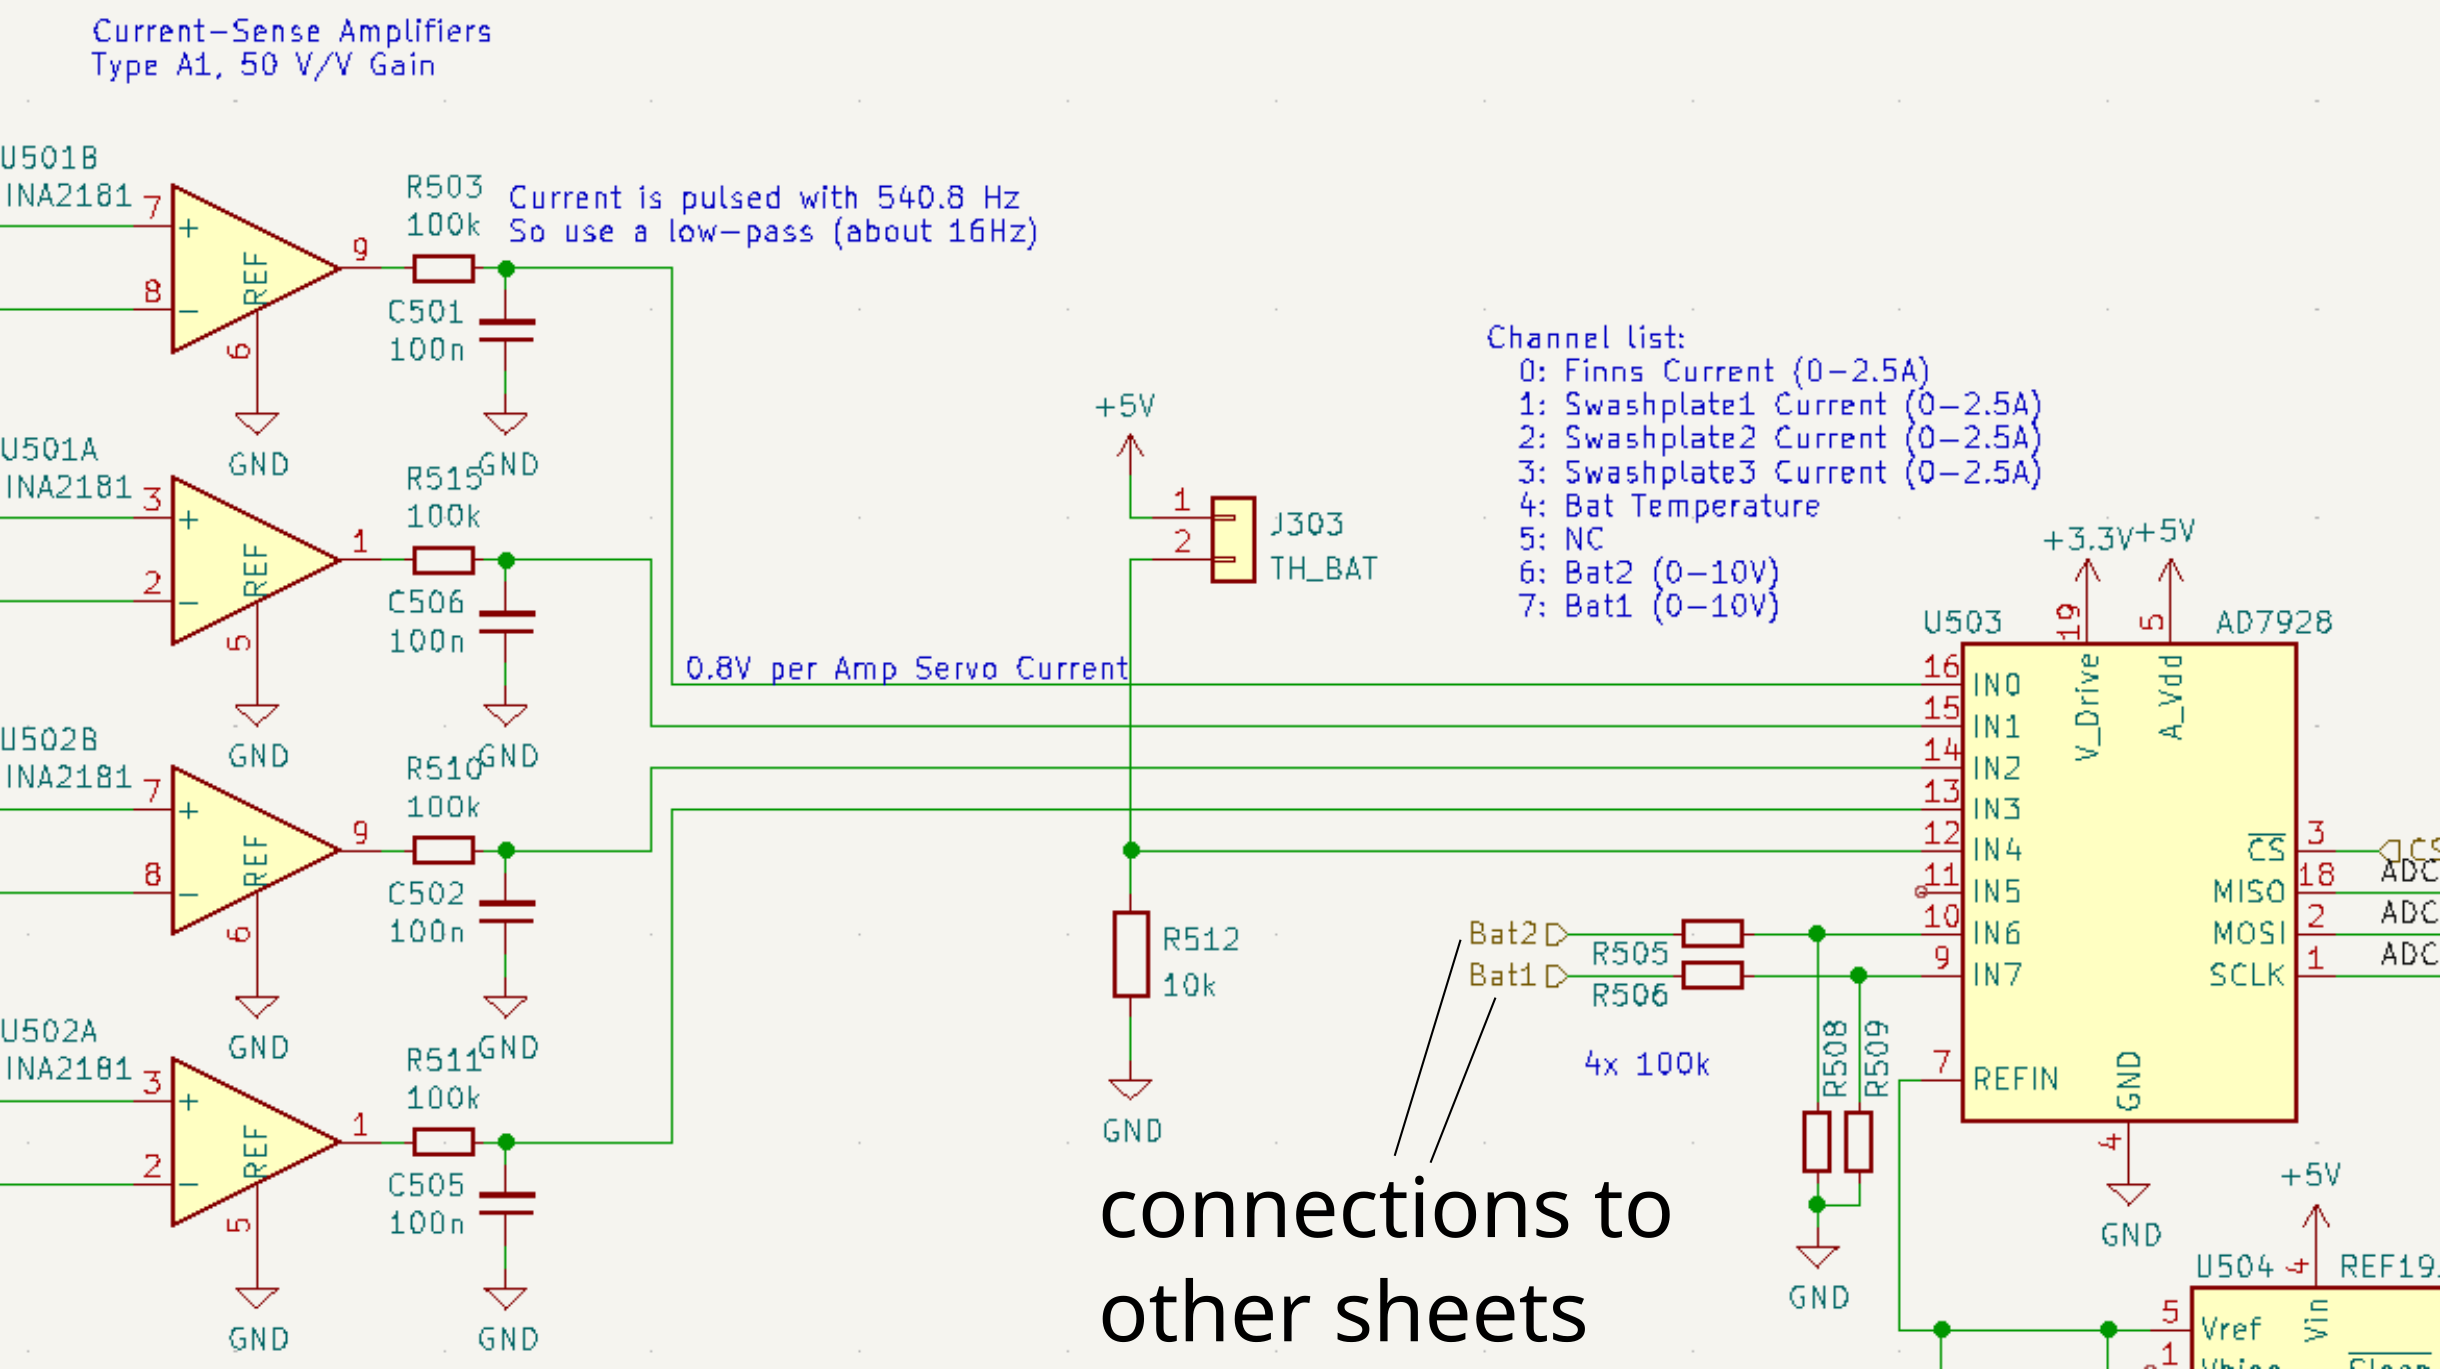
\includegraphics[width=\textwidth]{images/ex1-3.png} 
\end{frame}

\subsection{Schematic Conventions \& Etiquette}
\begin{frame}{Schematic Etiquette}
  Don't!\\
  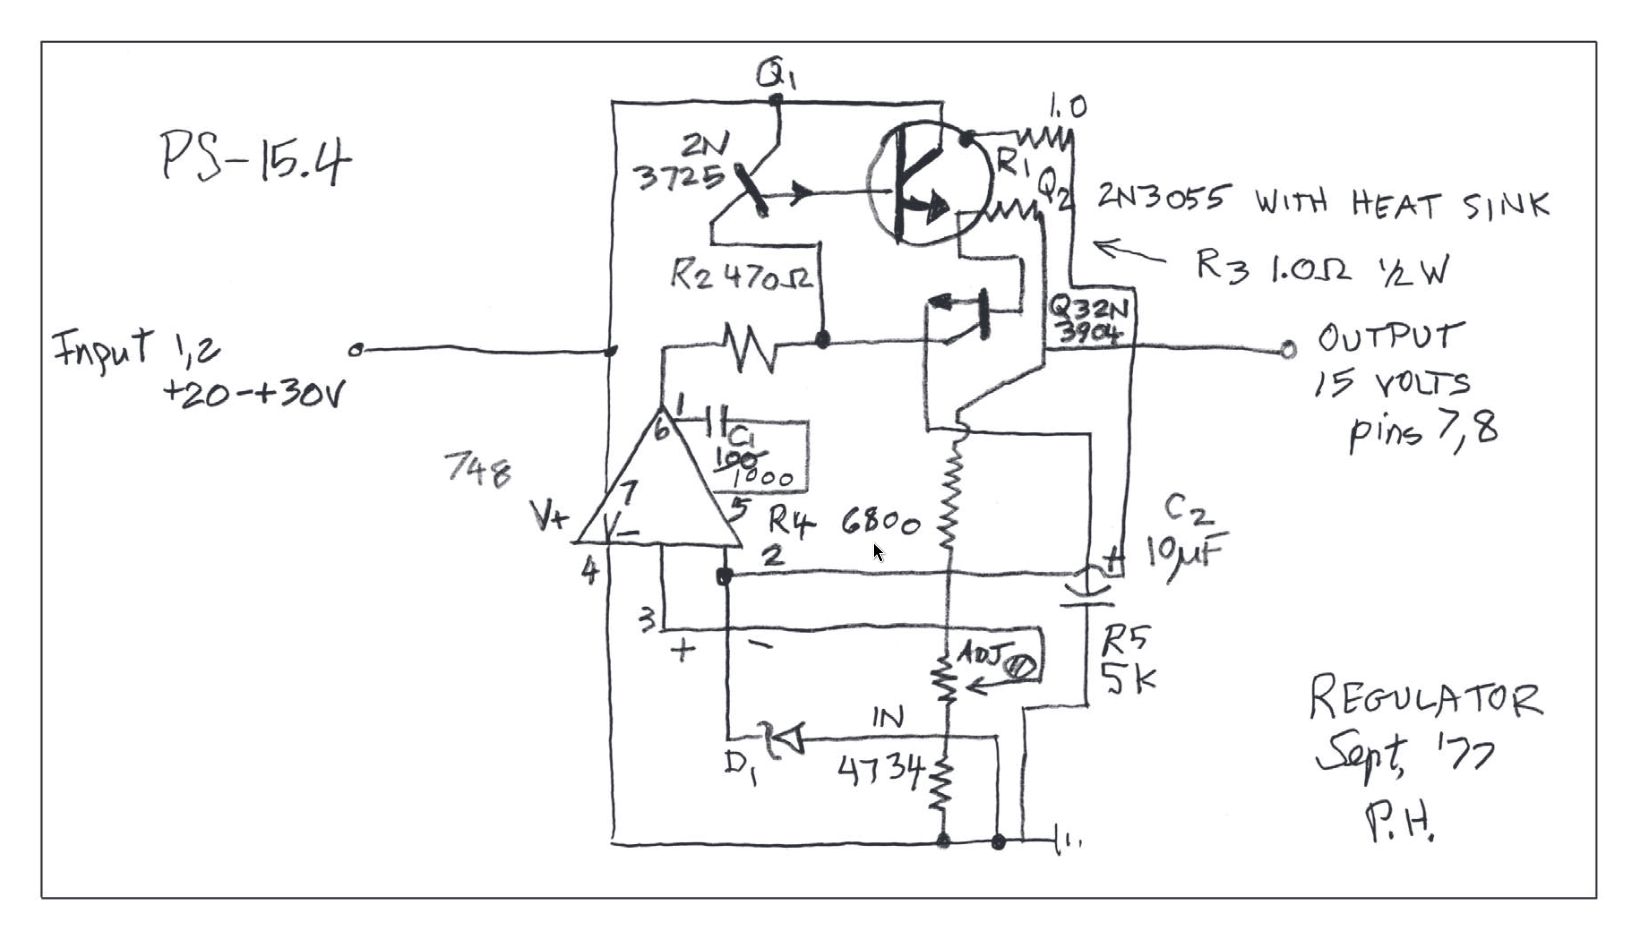
\includegraphics[width=\textwidth]{images/schematic-dont.png} 
\end{frame}

\begin{frame}{Schematic Etiquette}
  Do!\\
  \centering
  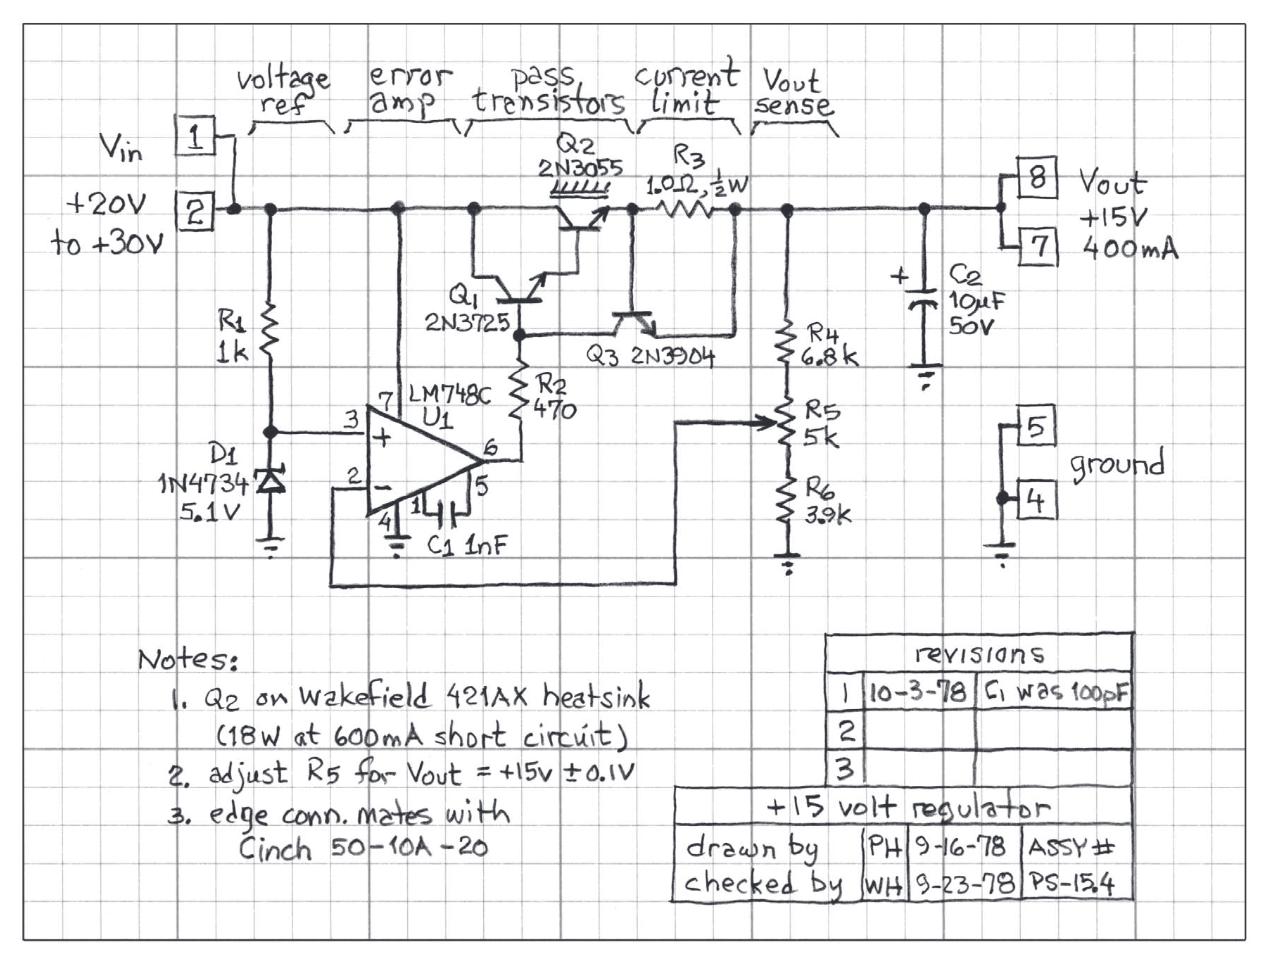
\includegraphics[width=0.9\textwidth]{images/schematic-do.png} 
\end{frame}

\begin{frame}{Schematic Etiquette}
  \begin{itemize}
    \item Drawing nice schematics comes with years of experience, but it's worth it.\\
    \item Debugging a neatly drawn circuit is 100x more fun than debugging a confusing rat's nest.\\
    \pause
    \item It's the same as debugging the horrible spaghetti code you wrote 2 years ago.
    \pause
    \item But I'm still messy sometimes, especially if it's a quick\&dirty first prototype ;)
  \end{itemize}
\end{frame}

\begin{frame}{Schematic Etiquette}
  For the love of God, DON'T!\\
  \centering
  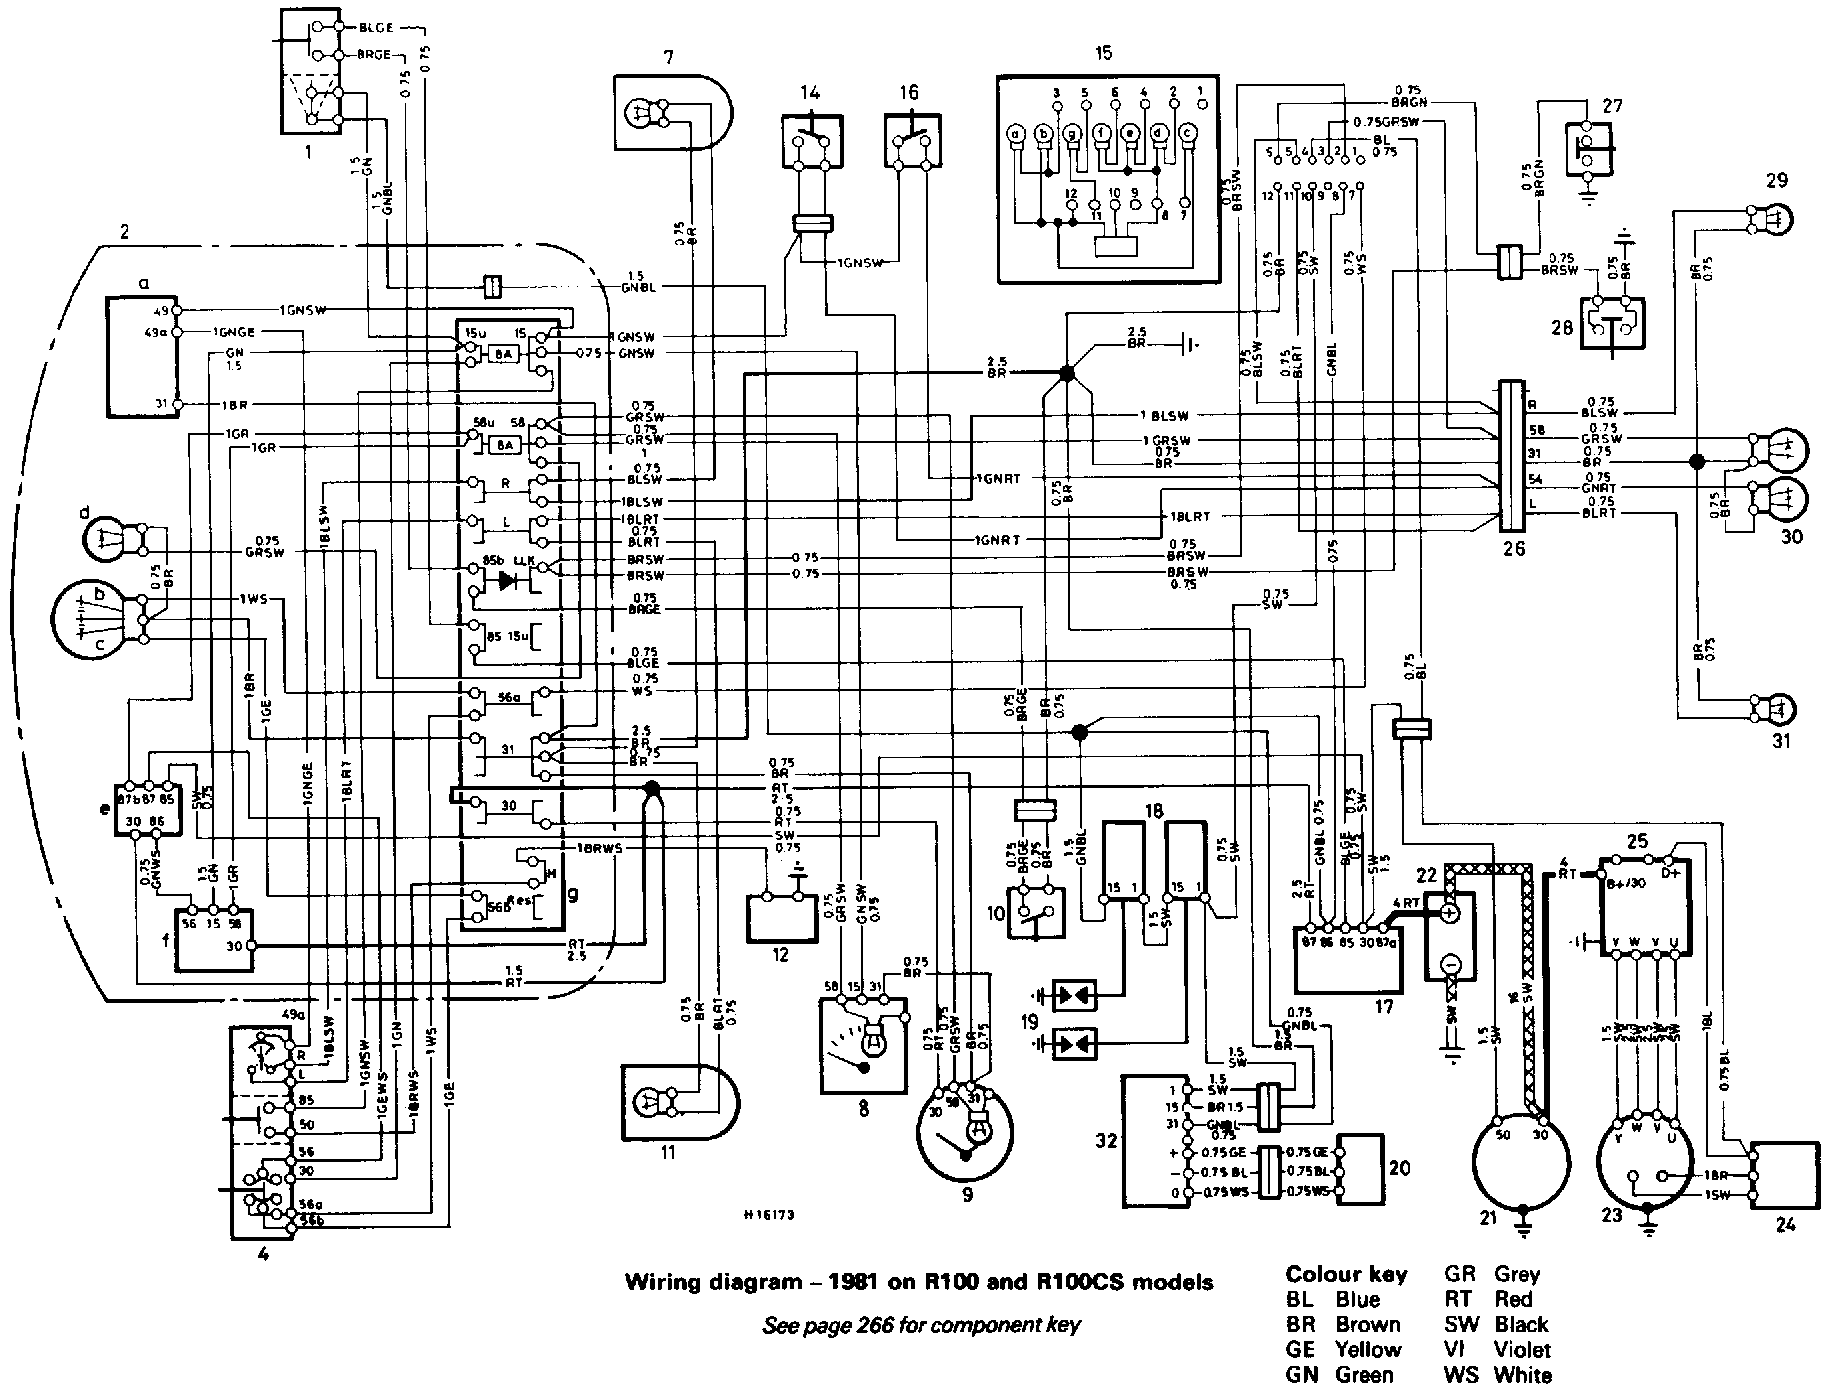
\includegraphics[width=0.9\textwidth]{images/bad-schematic.png}
\end{frame}

\subsection{Task 1: Designing a Light Sensor}

\begin{frame}{Let's begin!}
  \begin{itemize}
    \item Open KiCad by clicking on this icon: \raisebox{-.35\height}{
\includegraphics[width=0.1\textwidth]{images/kicad-icon.png}}
    \item Create a new project: \raisebox{-0.9\height}{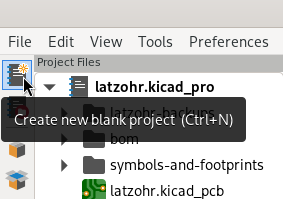
\includegraphics[height=3cm]{images/create-new-project.png}}
    \item Open the Schematic Editor!
  \end{itemize}
\end{frame}

\begin{frame}{Schematic Commands}
  \hspace{-0.5cm}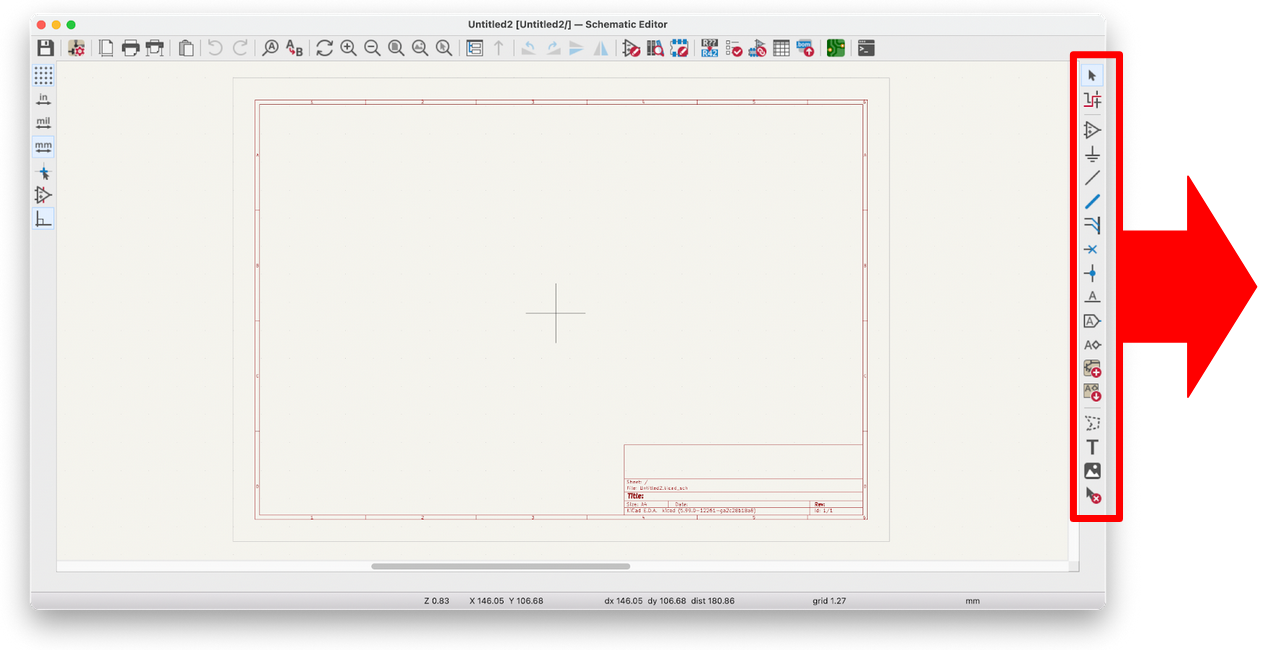
\includegraphics[width=0.8\textwidth]{images/eeschema.png}
  \raisebox{-2cm}{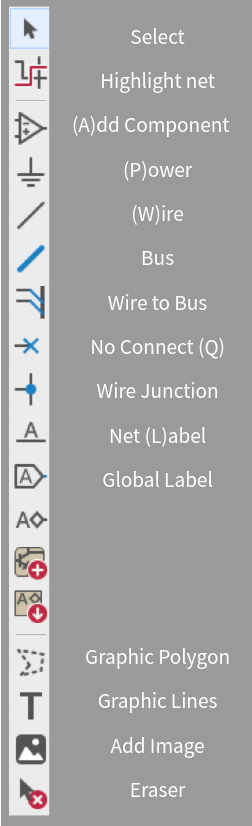
\includegraphics[height=.9\textheight]{images/eeschema-commands.png}}
\end{frame}

\begin{frame}{Our Goal}
  Our goal is to replicate this schematic:

  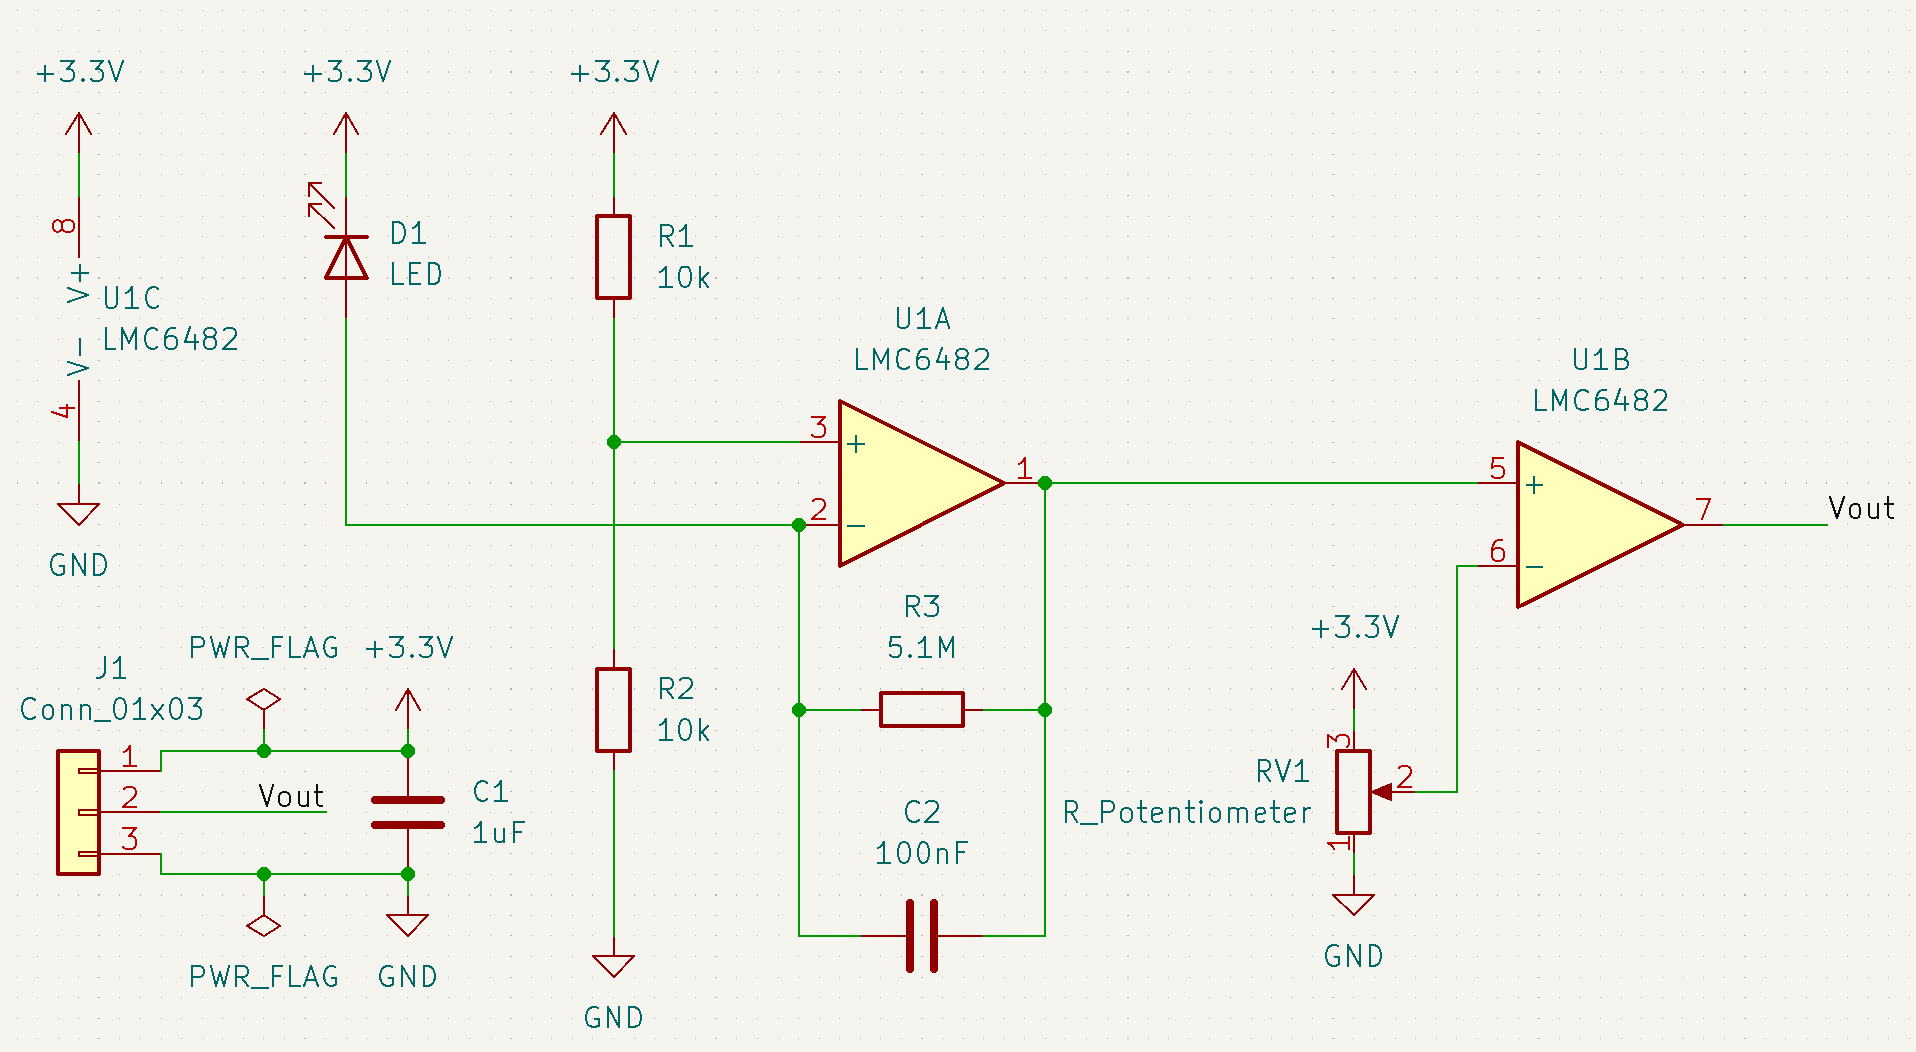
\includegraphics[width=\textwidth]{images/schematic-goal.png}

  It's a light detector!
\end{frame}

\begin{frame}{Wait a Moment}
  \begin{center}
  
\includegraphics[width=0.45\textwidth]{images/thats-illegal.png}
  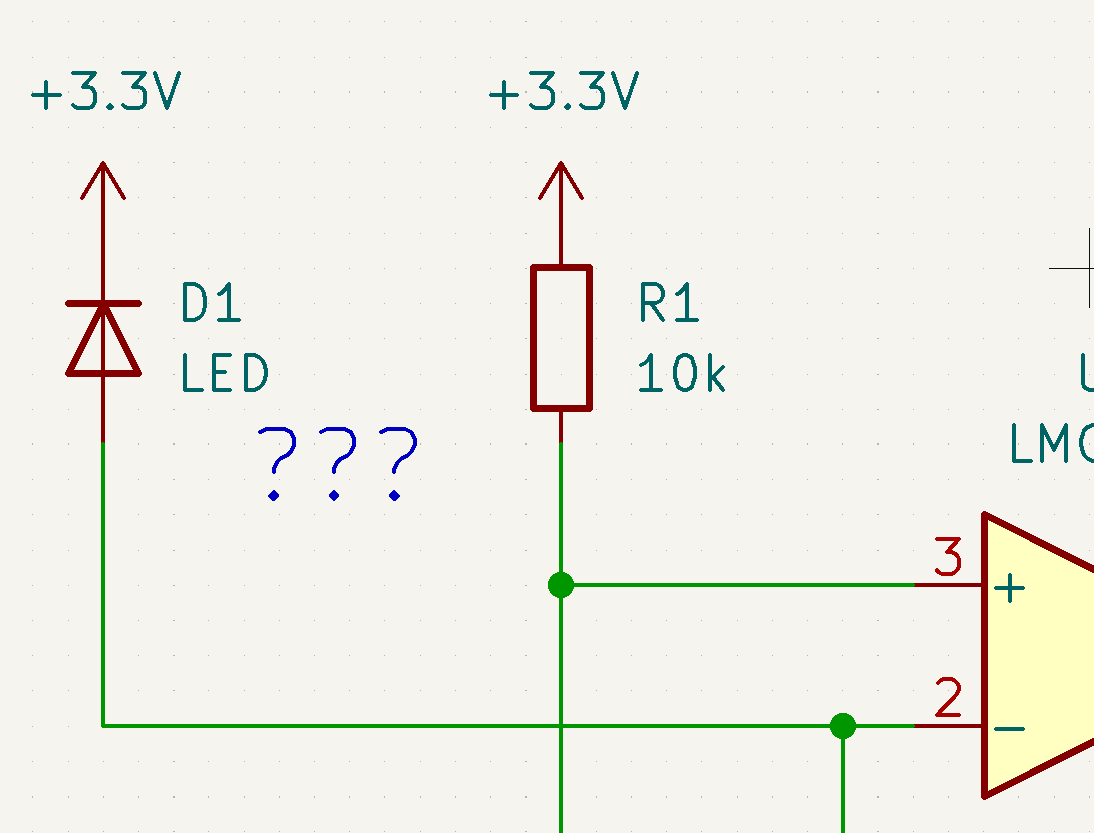
\includegraphics[width=0.4\textwidth]{images/diode-wrong-way.png}\\
  \end{center}
  \pause
  \begin{columns}
    \column{0.6\textwidth}
      Isn't this LED the wrong way around?\\
    \vspace{0.2cm}
      Yeah, but we're cheating a bit. A LED can also work as a light sensor.
      It generates a negative voltage when light shines on it!
    \column{0.4\textwidth}
    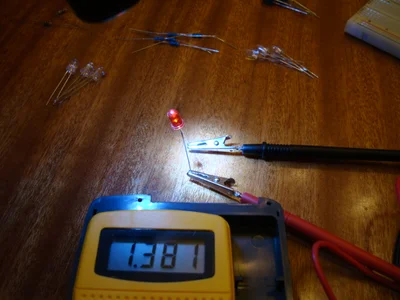
\includegraphics[width=\textwidth]{images/led-as-sensor.png}
  \end{columns}
\end{frame}

\begin{frame}{First Component}
  We will first place the diode \textbf{D1}
  \begin{itemize}
    \item Press the shortcut \textit{a} to \textbf{a}dd a component and enter \textit{led} into the search bar
    \item Press \textit{r} to \textbf{r}otate
    \item If happy, click anywhere to place the component
  \end{itemize}

  \vfill
  \begin{columns}
    \column{0.6\textwidth}
    \begin{quote}
      Use the \sout{force} shortcuts, Luke!

    {\normalfont \scriptsize - Obi-Wan, probably}
    \end{quote}
    \column{0.4\textwidth}
    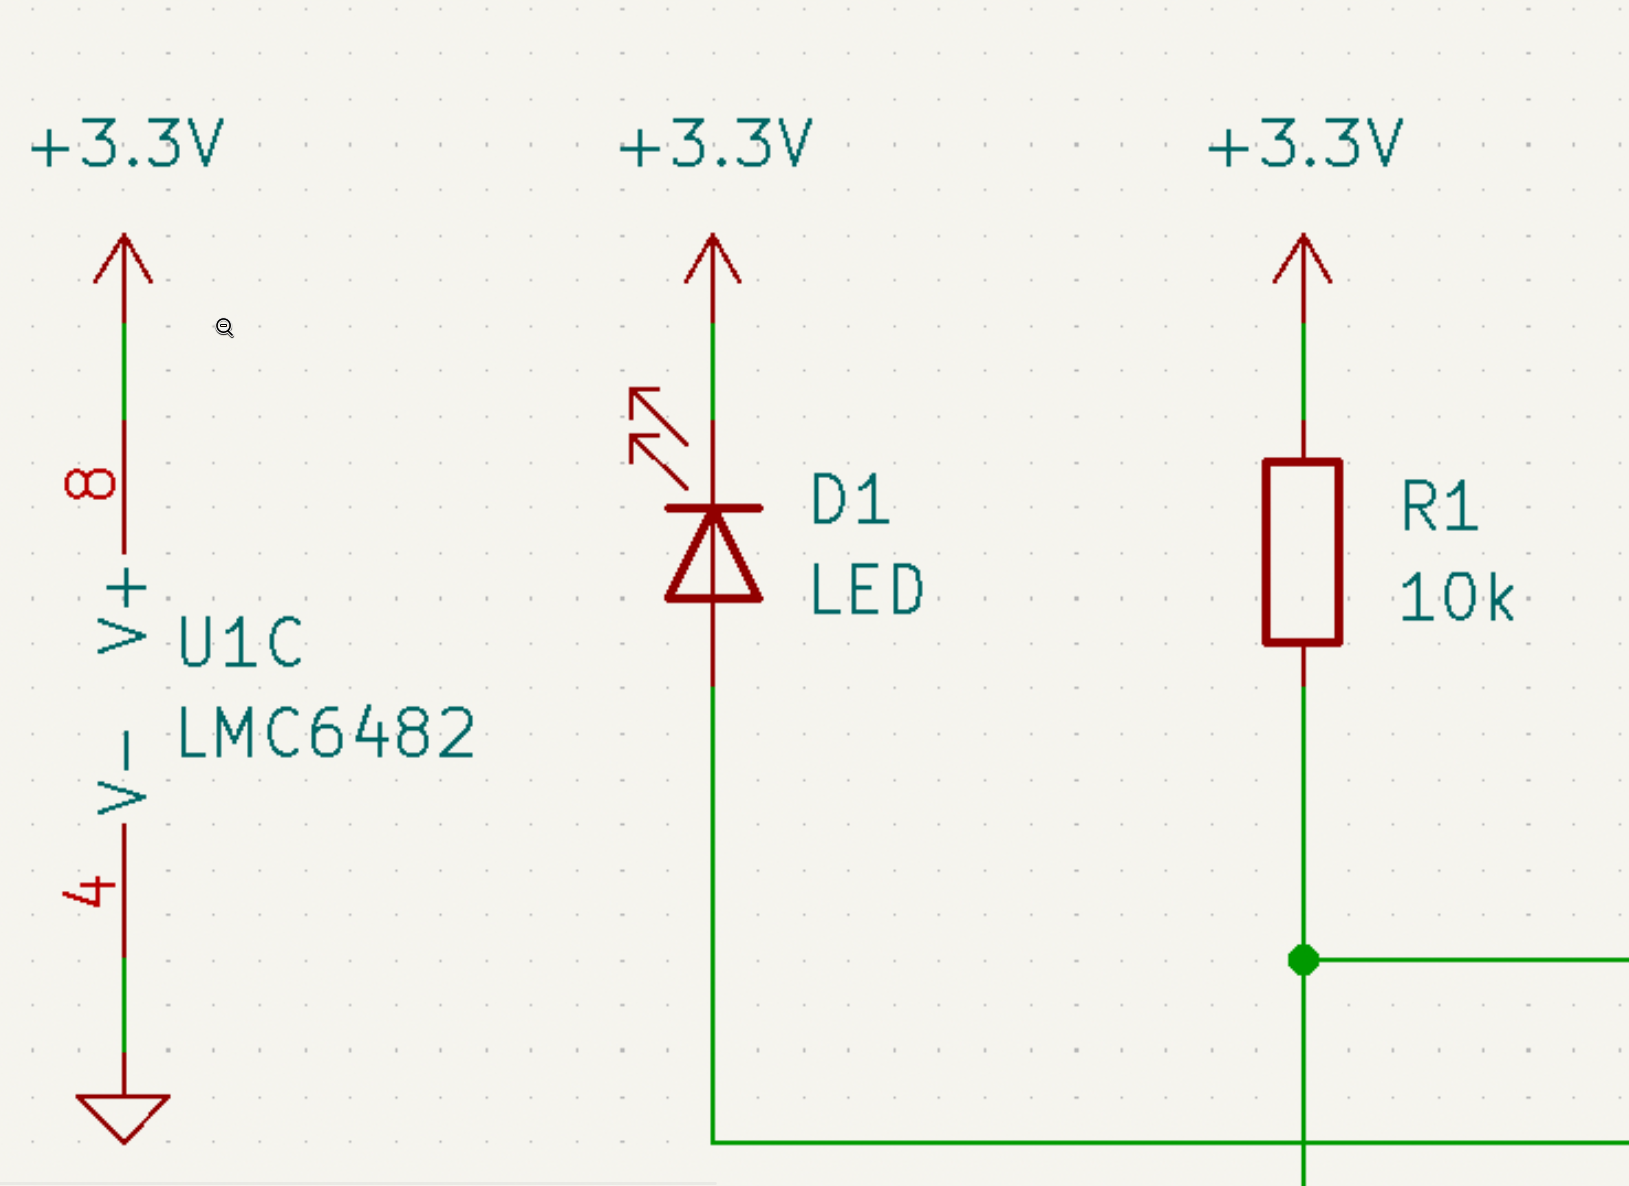
\includegraphics[width=\textwidth]{images/first-steps.png}
  \end{columns}
\end{frame}

\begin{frame}{First Component}
  Now repeat those steps for the resistor \textbf{R1}.

  \begin{itemize}
    \item Again, add with \textit{a} and type \textit{r} for resistor.
    \item Unhappy with the placement? Press \textit{m} to \textbf{m}ove a component
  \end{itemize}

  \vfill
  \begin{columns}
    \column{0.6\textwidth}
    \begin{quote}
      Use the \sout{force} shortcuts, Luke!

    {\normalfont \scriptsize - Obi-Wan, probably}
    \end{quote}
    \column{0.4\textwidth}
    \includegraphics[width=\textwidth]{images/first-steps.png}
  \end{columns}
\end{frame}

\begin{frame}{Multi-Symbol Components}
  \begin{itemize}
    \item Now we add the operational amplifiert (OpAmp).
    \item Add with \textit{a} and start typing \textit{LMC6482}
    \item KiCad will allow you to place multiple components! Why could that be?
    \item Hint: Look up the \href{http://www.ti.com/lit/ds/symlink/lmc6482.pdf}{LMC6482's datasheet}
  \end{itemize}
\end{frame}

\begin{frame}{Placing all Components}
  \vspace{-0.2cm}
  In total we need:
  \vspace{-0.2cm}
  \begin{itemize}
    \item 2 capacitors (C or C\_Small)
    \item 3 resistors (R or R\_Small)
    \item a LED part symbol (LED)
    \item a potentiometer part symbol (R\_Potentiometer)
    \item a 1x3 connector part symbol (CONN\_01x03) - should be listed as generic
  \end{itemize}
  \centering
  \includegraphics[width=\textwidth]{images/schematic-all-components.png}
\end{frame}

\begin{frame}{Adding Wires}
  \begin{itemize}
    \item The values for the resistors and capacitors will be blank (R, C), ignore this for now
    \pause
    \item Wire up your components! Press \textit{w} for \textbf{w}ire to activate the wire tool and press \textit{Esc} to go back to the selection tool.
    \item Repeat until the schematic is fully captured.
    \pause
    \item Drag placed wires by selecting or hovering over them and pressing \textit{g} for \textbf{g}rab.
    \item Delete segments by selecting or hovering over and pressing \textit{Backspace} or \textit{Del}, or right-click the wire for more options.
    \item To create a wire that does not connect to a component on one end
  (floating wire), double-click where you want the wire to end.
    
  \end{itemize}
\end{frame}

\begin{frame}{Placing Wires}
  It should look something like this:
  \includegraphics[width=\textwidth]{images/schematic-wires.png}
\end{frame}

\begin{frame}{Adding Labels}
  \includegraphics[width=\textwidth]{images/schematic-labels.png}
\end{frame}

\begin{frame}{Adding Labels}
  To add labels (the 'Vout' label shown above), press \textit{L} and type in the
  name of your label. Labels connect two or more nodes together without
  actually drawing the wire on screen. They are basically magic wire tunnels
  linked by name.

  \centering
  \includegraphics[width=0.6\textwidth]{images/underground-belt.png}
\end{frame}

\begin{frame}{Adding Power Ports}
  Now add power symbols to your schematic!
  \begin{itemize}
    \item We need \textit{GND} and \textit{+3.3V}
    \item It may be easier to duplicate components, instead of adding them separately. Try out 'Ctrl+C' and 'Ctrl+V'! ('Cmd+C' and 'Cmd+V' for Mac)
  \end{itemize}
  
  \centering
  \includegraphics[width=\textwidth]{images/schematic-power-symbols.png}
\end{frame}

\begin{frame}{Adding Power Flags}
  Next, add power flags to the schematic. Again, we can duplicate the first flag.\\

  \vfill
  \begin{quote}
  Power flags serve to tell the Electrical Rules Checker (ERC) in subsequent steps that the pin or wire is connected to power even if a power source isn't specified.
  \end{quote}

  \includegraphics[width=0.4\textwidth]{images/power-flags.png}
\end{frame}

\begin{frame}{Assign Value}
  Assign values to components. The easiest way to do this is to select or hover
  over the component and press \textit{V}. You can also double-click the component to
  open its properties or right-click and open 'Properties'.
  
  Type the appropriate value. Omit units for resistors but include units for
  capacitors and inductors (F for farads, H for Henries, etc.). For example, a
  \SI{1}{\kilo\ohm} resistor value would simply be 1k and a \SI{1}{\nano\farad} capacitor value would be 1nF.
\end{frame}

\begin{frame}{Our Goal}
  Any problems?

  \includegraphics[width=\textwidth]{images/schematic-goal.png}
\end{frame}

\begin{frame}{Hell Yeah!}
  \centering
  \includegraphics[width=0.6\textwidth]{images/beginning-to-believe.png}
\end{frame}

\subsection{From Schematic to Physical Components}

\begin{frame}{Assigning Footprints}
  We have described our circuit in a way the computer and humans (hopefully) understand. Congratulations!
  Now we need to tell KiCad how these abstract components look in the real world. Or at least, how they will look on the PCB.
  This representation is called a footprint.

  \centering
  \includegraphics[width=0.6\textwidth]{images/footprints.jpg}
\end{frame}

\begin{frame}{What footprint to choose?}
  \begin{columns}
    \column{0.48\textwidth}
    \includegraphics[width=\textwidth]{images/resistor-tht-vs-smd.png}
    \column{0.48\textwidth}
    \includegraphics[width=\textwidth]{images/resistor-footprints.png}
  \end{columns}
\end{frame}

\begin{frame}{SMD Footprint Codes}

  \begin{columns}
    \column{0.45\textwidth}
    EIA footprint codes:
    \includegraphics[width=\textwidth]{images/EIA-codes.png}
    \column{0.55\textwidth}
    \includegraphics[width=\textwidth]{images/0402-resistor.png}
  Don't order 0402 components for your first project. You won't be happy.\\
  1206 or 0805 are beginner-friendly, but you still need a good pair of tweezers.
  \end{columns}
\end{frame}

\begin{frame}{Size Matters}
  \centering
  \includegraphics[width=0.7\textwidth]{images/size-matters1.png}
  \includegraphics[width=0.5\textwidth]{images/size-matters2.png}
\end{frame}

\begin{frame}{Imperial vs Metric footprints}
  \centering
  \includegraphics[width=0.8\textwidth]{images/imperial-metric-mixup.png}

  I know it hurts, but we use \textbf{imperial} footprint codes to avoid mixups!
  Or even better, name both: \texttt{Resistor\_SMD:R\_0603\_1608Metric}
\end{frame}

\begin{frame}{Assigning Footprints}
  \begin{center}
    \includegraphics[width=0.9\textwidth]{images/symbol-to-footprint.png}
  \end{center}
\end{frame}

\begin{frame}{Assigning Footprints}
  We will now assign footprints to all components.\\
  Go to \textit{Tools > Assign Footprints}, it should look like this:\\
  \includegraphics[width=\textwidth]{images/footprint-menu.png}
\end{frame}

\begin{frame}{Using the Assignment Tool}
  Activate the first two footprint filters. This will filter out footprints:
  \begin{itemize}
    \item That are in the same \textit{category} as your symbol (e.g. show only resistor footprints)
    \item That have the same \textit{pin count} as your symbol (e.g. show only footprints with 2 pins)
  \end{itemize}
  \pause
  These are some suggested footprints, but feel free to choose your own!
  \includegraphics[width=\textwidth]{images/footprint-selection.png}
\end{frame}

\section{PCB Layout}

\subsection{The PCB Editor}

\begin{frame}{PCB Editor}
  Now open the PCB editor!\\
  \includegraphics[width=0.4\textwidth]{images/open-pcb-editor.png}\\
  \pause
  We want to import the changes from the schematic into our PCB editor:\\
  \includegraphics[width=0.4\textwidth]{images/update-changes-from-schema.png}
\end{frame}

\begin{frame}{Component Distribution}
  Just like in the schematic we can move components with \textit{m} and rotate them with \textit{r}. Try to position everything in a manner that makes sense and avoid to many crossing blue lines.\\
  \vspace{2cm}
  \begin{quote}
    Pro-Tip: The OpAmp is the most complex component. Put it in the middle.
  \end{quote}
\end{frame}

\begin{frame}{Component Distribution}
  \centering
  The result could look somewhat like this:
  \includegraphics[width=0.9\textwidth]{images/distributed-components.png} 
\end{frame}

\subsection{Designing the Board}

\begin{frame}{Routing}
  Now starts the routing. Press \textit{x} over any pad to start drawing a trace. The corresponding pads should be highlighted:
  \begin{center}
    \includegraphics[width=0.9\textwidth]{images/routing.png} 
  \end{center}
\end{frame}

\begin{frame}{Routing}
  \begin{itemize}
    \item You can delete tracks with \textit{Del} (\textit{Entf})
    \item Don't worry about the GND connections. We'll do them last!
    \item You may realize that one layer is not enough. You can switch between layers with \textit{Page Up} and \textit{Page Down} (\textit{Bild~↑}/\textit{Bild~↓})
    \item You can also jump between layers with \textit{v}. While routing, \textit{v} places a via!
  \end{itemize}
  \begin{center}
    \includegraphics[width=0.45\textwidth]{images/placing-via.png}
  \end{center}
\end{frame}

\begin{frame}{Routing}
  Did everything work out?\\
  \includegraphics[width=0.9\textwidth]{images/all-routed.png}
\end{frame}

\begin{frame}{Board Outline}
  We need to define the board outline. For this, switch to the layer \texttt{Edge.Cuts} and use the rectangle or line tool:
  \begin{center}
    \includegraphics[width=0.4\textwidth]{images/add-board-outline.png}
  \end{center}
\end{frame}

\begin{frame}{Board Outline}
  Outlines can be really complicated, but a rectangle is enough for now.\\
  \begin{center}
    \includegraphics[width=0.6\textwidth]{images/complicated-outline.png}
  \end{center}
\end{frame}

\begin{frame}{Silkscreen Comments}
  By switching to the layer \texttt{F.Silkscreen} and using the text tool we can add \sout{helpful comments} memes to our PCB.
  \begin{center}
    \includegraphics[width=0.7\textwidth]{images/pcb-memes.png}
  \end{center}
\end{frame}

\begin{frame}{Preview Time}
  By pressing \textit{Alt + 3} we can view a 3D render of our board!\\
  \begin{center}
    \includegraphics[width=0.7\textwidth]{images/3d-preview.png}
  \end{center}
  \pause
  I'm missing the model of \texttt{RV1}, the potentiometer :(
\end{frame}

\begin{frame}{Ground Pour}
  Next we want to fill the remaining space on our board with a copper pour. Press this button to add a filled zone:
  \begin{center}
    \includegraphics[width=0.4\textwidth]{images/add-filled-zone.png}
  \end{center}
  \begin{itemize}
    \item Select both front and back layer
    \item Select the GND net
  \end{itemize}
\end{frame}

\begin{frame}{Ground Pour}
  \begin{center}
    \includegraphics[width=0.9\textwidth]{images/fill-zone.png}
  \end{center}
\end{frame}

\begin{frame}{Ground Pour}
  \begin{itemize}
    \item Draw a rectangle along the edge cut and double click to end.
    \item Press \textit{b} to fill the copper pour.
  \end{itemize}

  \begin{center}
    \includegraphics[width=0.7\textwidth]{images/zones-filled.png}
  \end{center}
\end{frame}

\begin{frame}{Label your Pins!}
  We can use an amazing plugin to generate beautiful pin labels:
  \begin{center}
    \includegraphics[width=0.7\textwidth]{images/kibuzzard.png}
  \end{center}
\end{frame}

\begin{frame}{Label your Pins!}
  We can use an amazing plugin to generate beautiful pin labels:
  \begin{center}
    \includegraphics[width=0.7\textwidth]{images/kibuzzard.png}
  \end{center}
\end{frame}

\begin{frame}{Label your Pins!}
  \begin{center}
    \includegraphics[width=0.7\textwidth]{images/pin-label.png}
  \end{center}
\end{frame}

\begin{frame}{Ground Pour}
  A ground pour has multiple functions:
  \begin{itemize}
    \item Almost everything needs a ground connection, so a complete pour is useful
    \item A hot component can dissipate heat with such a big copper area
    \item Every flowing current also has a return current. With a ground plane, the return path can be next to the trace which reduces electromagnetic emissions
  \end{itemize}
\end{frame}

\subsection{Prepare for Manufacturing}

\begin{frame}{Gerber Export}
  \textit{File > Fabrication Outputs > Gerbers}
  \begin{center}
    \includegraphics[width=0.7\textwidth]{images/gerber-export.png}
  \end{center}
  Don't forget the drill files!
\end{frame}

\begin{frame}{AISLER Export}
  Or alternatively use one of the available direct exports like the AISLER push plugin
  \begin{center}
    \includegraphics[width=0.8\textwidth]{images/aisler-export.png}
  \end{center}
\end{frame}

\section{Further Topics}

\begin{frame}{Further Topics}
  Whoop! We created our first PCB, you can be proud :)\\
  There are a lot of further topics which are interesting, these include:
  \begin{itemize}
    \item Library management
    \item Drawing your own symbols and footprints
    \item BOM (bill of material) management
    \item Finding components on Mouser/Digikey
    \item KiCad and Git integration
    \item Controlled-impedance routing/length matching
    \item How to interact with manufacturers\\
      \includegraphics[width=0.3\textwidth]{images/well-got-your-order.jpg}
  \end{itemize}
  \small
  Soooo, maybe Crash Course Part 2? I make no promises though
\end{frame}

\begin{frame}{Course Evaluation}
  This was the first time I did such a course, so please help me improve it!\\
  There are feedback forms, and I'd be really grateful to hear your opinions and constructive criticism to make this better :)

  \begin{center}
    \includegraphics[width=0.4\textwidth]{images/feedback.png}
  \end{center}
\end{frame}

\end{document}
